%%%%%%%%%%%%%%%%%%%%%%%%%%%%%%%%%%%%%%%%%%%%%%%%%%%%%%%%%%%%%%%%%%%%%%%%%%%%
% AGUJournalTemplate.tex: this template file is for articles formatted with LaTeX
%
% This file includes commands and instructions
% given in the order necessary to produce a final output that will
% satisfy AGU requirements. 
%
% You may copy this file and give it your
% article name, and enter your text.
%
%%%%%%%%%%%%%%%%%%%%%%%%%%%%%%%%%%%%%%%%%%%%%%%%%%%%%%%%%%%%%%%%%%%%%%%%%%%%
% PLEASE DO NOT USE YOUR OWN MACROS
% DO NOT USE \newcommand, \renewcommand, or \def, etc.
%
% FOR FIGURES, DO NOT USE \psfrag or \subfigure.
% DO NOT USE \psfrag or \subfigure commands.
%%%%%%%%%%%%%%%%%%%%%%%%%%%%%%%%%%%%%%%%%%%%%%%%%%%%%%%%%%%%%%%%%%%%%%%%%%%%
%
% All questions should be e-mailed to latex@agu.org.
%
%%%%%%%%%%%%%%%%%%%%%%%%%%%%%%%%%%%%%%%%%%%%%%%%%%%%%%%%%%%%%%%%%%%%%%%%%%%%
%
% Step 1: Set the \documentclass
%
% There are two options for article format:
%
% 1) PLEASE USE THE DRAFT OPTION TO SUBMIT YOUR PAPERS.
% The draft option produces double spaced output.
% 
% 2) numberline will give you line numbers.

%% To submit your paper:
%\documentclass[draft,linenumbers]{agujournal}
%\draftfalse

%% For final version.
\documentclass{agujournal}
\usepackage{url}
% Now, type in the journal name: \journalname{<Journal Name>}

% ie, \journalname{Journal of Geophysical Research}
%% Choose from this list of Journals:
%
% JGR-Atmospheres
% JGR-Biogeosciences
% JGR-Earth Surface
% JGR-Oceans
% JGR-Planets
% JGR-Solid Earth
% JGR-Space Physics
% Global Biochemical Cycles
% Geophysical Research Letters
% Paleoceanography
% Radio Science
% Reviews of Geophysics
% Tectonics
% Space Weather
% Water Resource Research
% Geochemistry, Geophysics, Geosystems
% Journal of Advances in Modeling Earth Systems (JAMES)
% Earth's Future
% Earth and Space Science
%
%

\journalname{Journal of Advances in Modeling Earth Systems (JAMES)}


\begin{document}

%% ------------------------------------------------------------------------ %%
%  Title
% 
% (A title should be specific, informative, and brief. Use
% abbreviations only if they are defined in the abstract. Titles that
% start with general keywords then specific terms are optimized in
% searches)
%
%% ------------------------------------------------------------------------ %%

% Example: \title{This is a test title}

%\title{Coupling physical parameterizations to high-order element-based Galerkin dynamical cores; the division of an element}

%\title{A finite-volume physics grid for coupling to element-based high-order Galerkin dynamical cores; the division of an element}

%\title{A finite-volume physics grid for coupling to spectral-element dynamical cores; the division of an element}

%\title{Physical parameterizations, their grid, and element based high-order Galerkin methods}

\title{Exploring a lower resolution physics grid in CAM-SE-CSLAM}

%% ------------------------------------------------------------------------ %%
%
%  AUTHORS AND AFFILIATIONS
%
%% ------------------------------------------------------------------------ %%

% Authors are individuals who have significantly contributed to the
% research and preparation of the article. Group authors are allowed, if
% each author in the group is separately identified in an appendix.)

% List authors by first name or initial followed by last name and
% separated by commas. Use \affil{} to number affiliations, and
% \thanks{} for author notes.  
% Additional author notes should be indicated with \thanks{} (for
% example, for current addresses). 

% Example: \authors{A. B. Author\affil{1}\thanks{Current address, Antartica}, B. C. Author\affil{2,3}, and D. E.
% Author\affil{3,4}\thanks{Also funded by Monsanto.}}

\authors{A.R. Herrington\affil{1}\thanks{Stony Brook, New York}, P.H. Lauritzen\affil{2}, K.A. Reed\affil{1}, S. Goldhaber\affil{2}, Mark A. Taylor\affil{3}}

 \affiliation{1}{School of Marine and Atmospheric Sciences, Stony Brook University, Stony Brook, New York}
 \affiliation{2}{National Center for Atmospheric Research, Boulder, Colorado, USA}
 \affiliation{3}{Sandia National Laboratories, Albuquerque, New Mexico, USA}

%% Corresponding Author:
% Corresponding author mailing address and e-mail address:

% (include name and email addresses of the corresponding author.  More
% than one corresponding author is allowed in this LaTeX file and for
% publication; but only one corresponding author is allowed in our
% editorial system.)  

% Example: \correspondingauthor{First and Last Name}{email@address.edu}

\correspondingauthor{Adam R. Herrington}{adam.herrington@stonybrook.edu}

% Example: 
% \begin{keypoints}
% \item	List up to three key points (at least one is required)
% \item	Key Points summarize the main points and conclusions of the article
% \item	Each must be 100 characters or less with no special characters or punctuation 
% \end{keypoints}

\begin{keypoints}
\item Control volumes are defined to provide an isotropic representation of the numerics to the physics
\item Grid imprinting from the spectral-element method is eliminated, even in regions with steep terrain
\item The coarser physics grid does not degrade the effective resolution of the model
\end{keypoints}

%% ------------------------------------------------------------------------ %%
%
%  ABSTRACT
%
% A good abstract will begin with a short description of the problem
% being addressed, briefly describe the new data or analyses, then
% briefly states the main conclusion(s) and how they are supported and
% uncertainties. 
%% ------------------------------------------------------------------------ %%

%% \begin{abstract} starts the second page 

\begin{abstract}
The effects of using a separate grid for evaluating physical parameterizations (a `physics grid') in global atmospheric models has long been discussed. While very few modeling studies have had the capability to experiment with a separate physics grid, here the implementation of a coarser resolution physics grid into CAM-SE-CSLAM is described. The results of experiments using the lower resolution physics grid are compared to the conventional method in which the physics grid and dynamical core grid coincide. Through dividing the elements of CAM-SE-CSLAM into $2\times2$ control volumes, each volume has the same smoothness property and eliminates grid imprinting, even in regions with steep topography. The impact of the coarser resolution physics grid on the resolved scales of motion is analyzed across a range of dynamical core grid resolutions. The results demonstrate that the effective resolution of the model is not degraded through the use of a coarser resolution physics grid. Since the physics makes up about half the computational cost of the conventional CAM-SE-CSLAM configuration, the coarser physics grid may allow for significant cost savings with little to any downside.
\end{abstract}


%% ------------------------------------------------------------------------ %%
%
%  TEXT
%
%% ------------------------------------------------------------------------ %%

%this should be included in the next paper (physres)
%When introducing a physics grid separate from the dynamics grid the question arises of what the resolution of the physics grid should be compared to the dynamics grid. For example, Figure \ref{fig:physgrid-1d} shows physics grids with the same, coarser and finer resolution than the GLL dynamics grid. From linear stability and accuracy analysis of numerical methods, it is a common result that the shortest resolvable wavelengths are not accurately represented. Similar arguments can be made from analyzing total kinetic energy spectra \citep{S2011LNCSE}. One may therefore argue that only believable scales should be passed to the physical parameterizations \citep{LH1997MWR}, i.e. a coarser resolution physics grid. This concept was investigated in a spectral transform model by \cite{W1999T}. On the other hand, computing physics tendencies on a higher-resolution grid compared to the dynamical core may provide a better sampling of the atmospheric state, somewhat similar to the super-parameterization \citep{G2001JAS,GRL:GRL14999,SA2007ASL} and sub-columns{\footnote{\citet{gmdd-8-5041-2015} in the context of CAM}} \citep{subcolumn,JGRD:JGRD10481} concepts. This approach was taken by \cite{M2009T} in the context of vertical refinement. \cite{W2014PTRSL} found improved forecast scores by increasing the grid-point space resolution compared to the resolution in wave-number space for the spectral transform model at ECMWF. 

%Alternatively, one could combine the two ideas and compute the state of the atmosphere on a coarser resolution grid and then use sub-columns or super-parameterization. One thereby passes believable scales to the sub-grid scale model and thereby assumes that a statistical sampling, in the case of sub-columns, or a simplified cloud-resolving model, in the case of super-parameterization, provides a more accurate sub-grid-scale tendency than sampling the Galerkin basis functions over the sub-grid-scale. [Discuss \cite{W2014PTRSL}: spectral truncation and physics (physical) grid (see page 10; conclusions)]

%Separating physics and dynamics grids has been investigated in the context of spectral transform models by \citet{TELA:TELA0009}, in which the separation was performed by truncation in wavenumber space. Parts of the physical parameterizations (microphysics) were separated in \citet{JGRD:JGRD50711} and vertical grid separation was investigated in \citet{TELA:TELA394}. In this study we run all of the parameterization on the physgrid.

%In the context of spectral transform model \citet{TELA:TELA0009} held the physics forcing scale fixed while refining the horizontal resolution of the dynamical core. In the context of microphysics \citet{JGRD:JGRD50711} did a scale separation and \citet{TELA:TELA394} separated the vertical grids. While \citet{LH1997MWR} and \citet{TELA:TELA0009} separated scales truncation of the the wave transform, we here separate scales through integrating basis functions over control volumes and , contrary to \citet{JGRD:JGRD50711}, all of the physical parameterization computations are performed on the physgrid. We focus on horizontal separation of scales here.

\section{Introduction}\label{sec:intro}

Global atmospheric models fundamentally consist of two components. The dynamical core ({\em{dynamics}}), which numerically integrate the adiabatic equations of motion and tracer advection, and the physical parameterizations ({\em{physics}}), which compute the effects of diabatic and subgrid-scale processes (e.g., radiative transfer and moist convection) on the grid-scale. More out of convenience than anything else, the physics are evaluated on the dynamics grid, i.e., the physics grid and dynamics grid coincide. From linear stability and accuracy analysis of numerical methods, it is a common result that the shortest simulated wavelengths are not accurately represented by the dynamical core. Additionally, simulated downscale cascades result in an unrealistic collection of energy and/or enstrophy near the truncation scale, which may be observed from kinetic energy spectra in model simulations \citep{S2011LNCSE}. Some form of dissipation must be incorporated into models to mitigate these numerical artifacts near the grid scale \citep{JW2010LNCSE}. This numerical dissipation has no physical analogy \citep[although see][]{GMR2007}, and the grid-scale is therefore contaminated by numerous un-physical processes. The under-resolved nature of the grid-scale led \cite{LH1997MWR} to speculate whether the physics should be evaluated on a grid that is more reflective of the scales actually resolved by the dynamical core.

Exploring the impact of different physics grid resolutions have so far been limited to models employing the spectral transform method \citep{LH1997MWR,W1999T,W2014PTRSL}. \cite{LH1997MWR} argue that passing under-resolved states to the physics may be especially problematic in spectral transform models, since the physics are evaluated on a latitude-longitude transform grid, and contains more degrees of freedom than the spectral representation to prevent aliasing of quadratic quantities. However, \cite{LH1997MWR} find that the spectral truncation of the physics tendencies damps errors that may result from passing an under-resolved state to the physics, although the extent to which these errors may still be present in the model is difficult to address. 

Another class of spectral-transform models evaluate the quadratic terms using semi-Lagrangian methods, which are implicitly diffusive, relaxing constraints on the resolution of the transform grid. \cite{W2014PTRSL} experimented with different transform grid resolutions and concluded that the standard high resolution quadratic grid actually improves forecast skill over the use of a lower-resolution transform grid. They suggests that increasing the resolution of the transform grid simulates a kind of sub-grid variability on the spectral state, which is thought to be under-represented in global atmospheric models \citep{S2005QJR}. This is in principle the purpose of ``super-parameterization," in which a cloud resolving model is embedded in each grid cell to approximate sub-grid variability, and improves both diurnal and sub-seasonal variability in the model \citep{RKAG2003BAMS}.

After the physics tendencies are transformed into spectral space, the tendencies may be truncated at any particular wave number. \cite{W1999T} conducted a pair of convergence tests using a global spectral transform model; a conventional convergence test and one in which the spectral truncation of the physics tendencies is held fixed and the resolution of the dynamical core increased. In contrast to the realistic weather forecasts of \cite{W2014PTRSL}, \cite{W1999T} run their model to equilibrium in an idealized climate configuration. When the physics and dynamics resolutions increase together, as in more typical convergence studies, the strength of the Hadley Cell increases monotonically with resolution. This sensitivity of Hadley Cell strength to horizontal resolution is a common result of global models at hydrostatic resolutions \citep[see][and references therein]{HR2017JCLIM}. But with the truncation wave number of physics tendencies held fixed, the Hadley Cell showed very little sensitivity to dynamical core resolution, resembling the solution for which the dynamics truncation wave number is equal to that of the lower resolution physics. 

\cite{HR2017JCLIM} speculate that the results of \cite{W1999T} indicate that the scales of motion resolved by the dynamical core are aliased to the lower resolution physics. It may be worth considering that if the resolution of the dynamics is reduced in response to a coarser physics grid, then the dynamics may be no better resolved on the coarser physics grid, compared with the conventional method of evaluating the physics and dynamics at the same resolution. The results of \cite{W1999T} and \cite{W2014PTRSL} do not provide evidence that a lower resolution physics grid reduces computational errors in spectral transform models, but again, this is a difficult problem to address, and seldom discussed in either study.  

Global spectral transform models, while remarkably efficient at small processor counts, do not scale well on massively parallel systems. High-order Galerkin methods are becoming increasingly popular in climate and weather applications due to their high-parallel efficiency, high-processor efficiency, high-order accuracy (for smooth problems), and geometric flexibility facilitating mesh-refinenment applications. High resolution climate simulations with NCAR's Community Atmosphere Model \citep[CAM;][]{CAM5} are typically performed using a continuous Galerkin dynamical core referred to as CAM-SE \citep[CAM Spectral Elements;][]{TES2008JPCS,DetAl2012IJHPCA,LetAl2018JAMES}. CAM-SE may be optionally coupled to a conservative, semi-Lagrangian tracer advection scheme for accelerated multi-tracer transport \citep[CAM-SE-CSLAM;][]{LTOUNGK2017MWR}. Tracer advection then evolves on an entirely separate, finite-volume grid which contains the same degrees of freedom as CAM-SE's quadrature node grid.

Element-based Galerkin methods are susceptible to grid-imprinting, and may need be considered when contemplating a particular physics grid \citep[][hereafter referred to as H18]{HL2018MWR}. Grid imprinting manifests at the element boundaries, since the global basis is least smooth ($C^{0}$; all derivatives are discontinuous) for quadrature nodes lying on the element boundaries, and the gradients (e.g., the pressure gradient) are systematically tighter producing local extremes. Through computing the physics tendencies at the nodal points, element boundary extrema is also observed in the physics tendencies. 

H18 has shown that through evaluating the physics on the finite-volume tracer advection grid in CAM-SE-CSLAM, element boundary noise is substantially reduced, although still problematic in regions of steep terrain, at low latitudes. Through integrating CAM-SE's basis functions over the control volumes of the finite-volume grid, element boundary extrema is additionally weighted by the $C^{\infty}$ solutions (i.e., the basis representation is infinitely smooth and all derivatives are continuous) that characterize the interior of the element, and the state is smoother. Additionally, in defining an area averaged state, the finite-volume physics grid is made consistent with assumptions inherent to the physics, and is more appropriate for coupling to other model components (e.g., the land model), which is typically performed using finite-volume based mapping algorithms.

The finite-volume grid of H18 is found through dividing the elements of CAM-SE's gnomic cubed-sphere grid with equally spaced, equi-angular coordinate lines parallel to the equi-angular element boundaries, such that there are $3\times 3$ control volumes per element (hereafter referred to as $pg3$; see Figure~\ref{fig:area-schematic}b). While a $3\times 3$ physics grid was chosen in order to have the same degrees of freedom as the dynamical core, the control volumes encompass a region of the element in which their proximity to the element boundaries are not equal. Therefore, not every control volume in an element has the same smoothness properties. This may be avoided through defining a physics grid in which the elements are instead divided into $2\times 2$ control volumes (hereafter referred to as $pg2$; see Figure~\ref{fig:area-schematic}a). The control volumes of the $pg2$ grid all have the same proximity to the element boundaries, and should mitigate the element boundary noise that remains in the $pg3$ grid, and shown in H18.

In this study, we test the hypothesis that the coarser, $pg2$ physics grid is effective at reducing spurious noise at element boundaries, particularly over regions of rough topography. In addition, the recent trend towards running models at ever higher resolutions is an almost prohibitive computational burden. As the physics are responsible for over half of the computational cost in CAM-SE \citep{LetAl2018JAMES}, the improvement in computational performance using a coarser resolution physics grid is potentially significant. However, any advantages of using a coarser physics grid need be weighed against any potential reduction in simulation quality, e.g., possible aliasing of the resolved scales of motion by the coarser grid, as suggested by the results of \cite{W1999T}. Section \ref{sec:methods} describes the implementation of the $pg2$ grid into CAM-SE-CSLAM. Section \ref{sec:results} provides the results of idealized model configurations to identify any changes in grid imprinting, or in the overall solution, compared with the $pg3$ configuration. Section \ref{sec:conclusions} provides a discussion of the results and conclusions.

\section{Methods}\label{sec:methods}

Separating dynamics, tracer and physics grids introduces the added complexity of having to map the state from dynamics and tracer grids to the physics grid; and mapping physics tracer increments back to the tracer grid and physics increments needed by the dynamical core to the dynamics grid (see Figure \ref{fig:overview}). The dynamics grid in the case of CAM-SE-CSLAM refers to the Gauss-Lobatto-Legendre (GLL) quadrature nodes used by the spectral-element method to solve the momentum equations for the momentum vector $(u,v)$, thermodynamics equation for temperature ($T$), continuity equation for dry air mass ($\frac{1}{g}p$), and continuity equations for water vapor and thermodynamically and inertially active condensates \citep[see, e.g., ][ for details]{LetAl2018JAMES}. By tracer grid we refer to the $pg3$ grid on which CSLAM performs tracer transport of water vapor, condensates and other tracers. Although water vapor and condensates are being advected by the CSLAM scheme on the $pg3$ grid, these quantities are also needed on the GLL grid for the momentum equations and thermodynamic equation. Transport of water variables is also performed by the spectral-element method on the GLL grid. To avoid decoupling of water species on the CSLAM and GLL grids, the GLL water species are overwritten by the CSLAM values every physics time-step. This is explained in detail in H18.

\begin{figure}[t]
\begin{center}
\noindent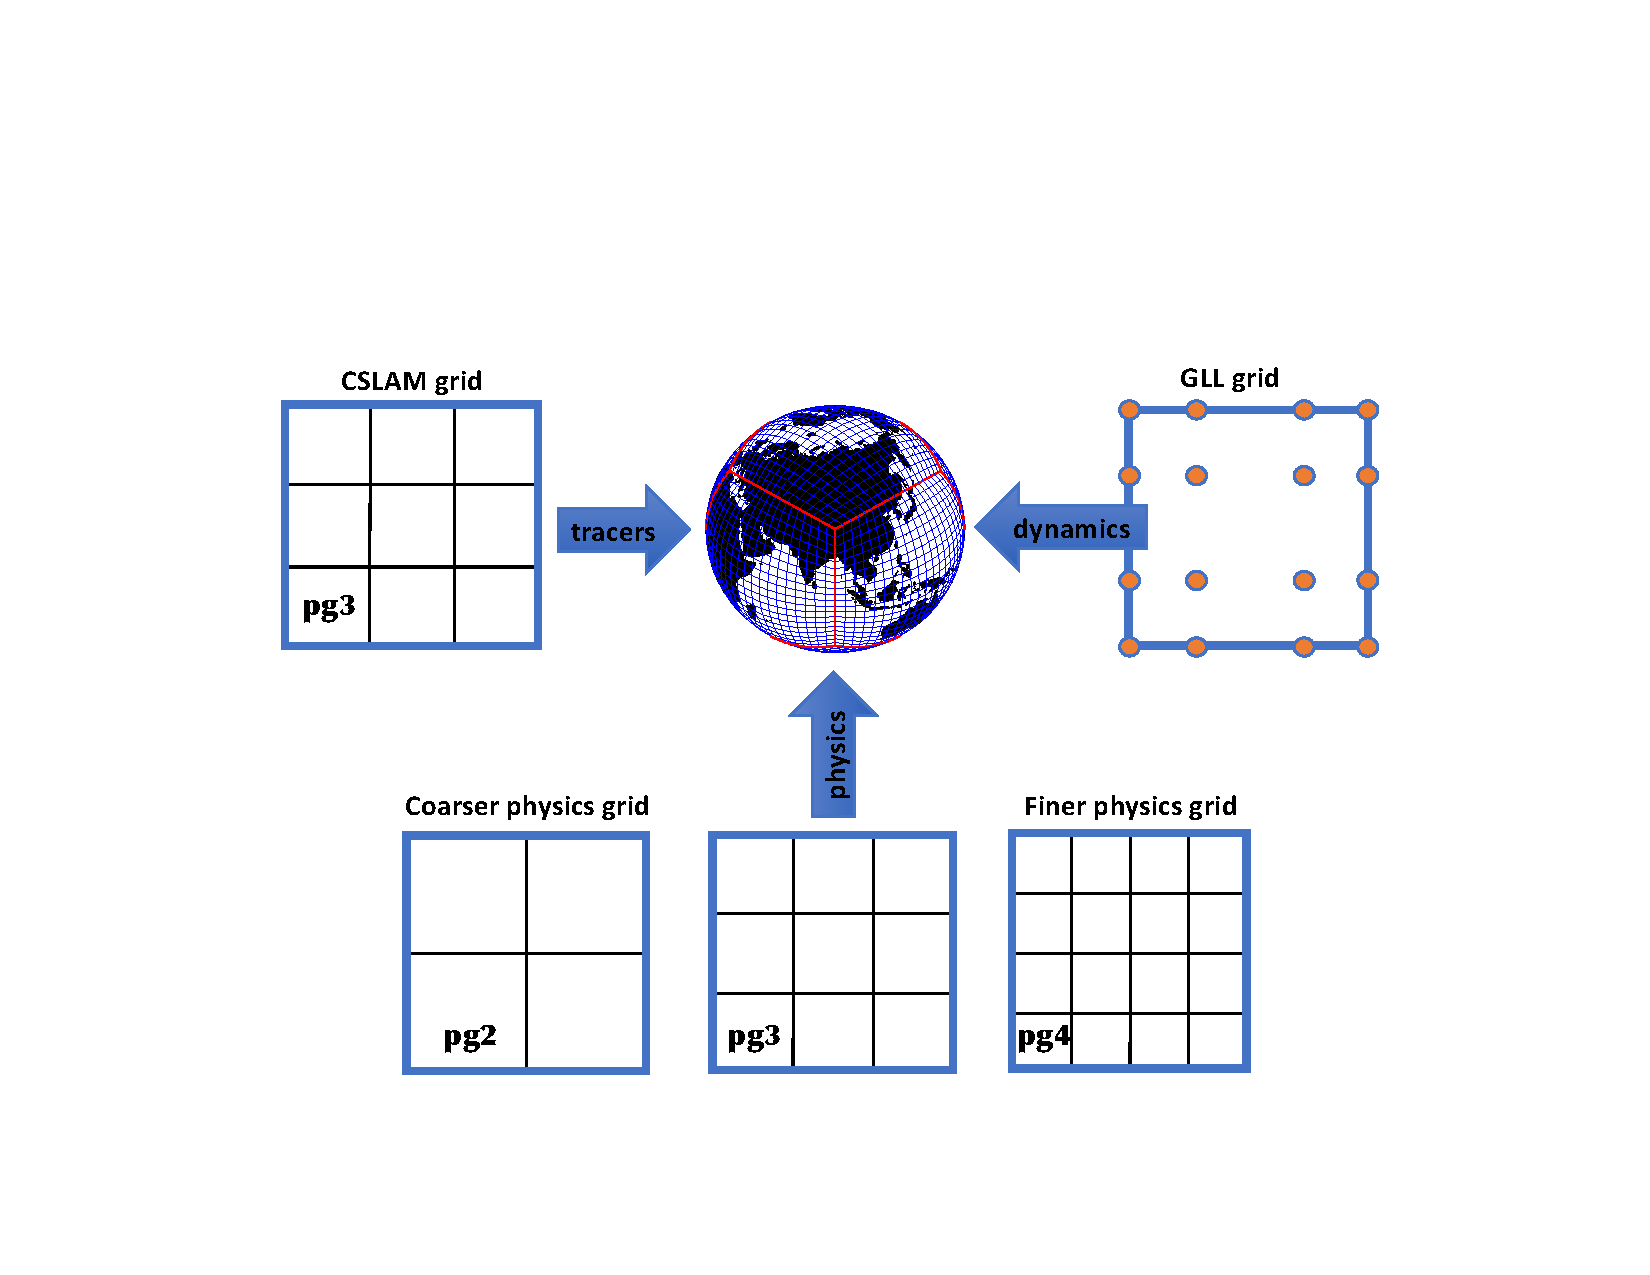
\includegraphics[width=30pc,angle=0]{figs/fig-overview.pdf}\\
\end{center}
\caption{An overview of the different grids in CAM-SE-CSLAM.}
\label{fig:overview}
\end{figure}

Similarly to the CAM-SE-CSLAM $pg3$ configuration, the dynamics state (momentum vector, temperature, dry pressure) must be mapped from the $GLL$ grid to the physics grid. Exactly the same algorithms as used in the $pg3$ configuration apply, i.e. momentum components are interpolated by evaluating the internal Lagrange basis functions (used in the spectral-element method) at the equi-angular (gnomonic) center of the $pg2$ cells and the Lagrange basis function representations of temperature and pressure are integrated over the $pg2$ control volumes. See H18 for details.

As compared to the $pg3$ configuration, the extra complication with the $pg2$ setup is that the tracer grid does not coincide with the physics grid, i.e. the tracer state needs to be mapped from the CSLAM grid ($pg3$) to the physics grid ($pg2$), and tracer increments computed by physics must be mapped from the physics grid back to the CSLAM grid. In order to describe the mapping algorithms between the grids some notation needs to be introduced.

The mapping algorithms are applied to each element $\Omega$ (with spherical area $\Delta \Omega$) so without loss of generality consider one element. Let $\Delta A^{(pg2)}_k$ and $\Delta A^{(pg3)}_\ell$ be the spherical area of the physics grid cell $A^{(pg2)}_k$ and CSLAM control volume $A^{(pg3)}_\ell$, respectively. The physics grid cells and CSLAM cells, respectively, span the element, $\Omega$, without gaps or overlaps
\begin{eqnarray}
\cup_{k=1}^{nphys^2}A^{(pg2)}_k=\Omega \text{ and } A^{(pg2)}_k \cap A^{(pg2)}_\ell = \emptyset \quad \forall k\ne \ell,\\
\cup_{k=1}^{nc^2}A^{(pg3)}_k=\Omega \text{ and } A^{(pg3)}_k \cap A^{(pg3)}_\ell = \emptyset \quad \forall k\ne \ell,
\end{eqnarray}
where $nc=3$ is the CSLAM grid resolution parameter and $nphys=2$ is the physics grid resolution parameter (following the Fortran code base), although the methods described here are valid for any arbitrary integer $nphys$ (e.g., $nphys=4$ is shown in Figure~\ref{fig:overview}). The overlap areas between the $k$-th physics grid cell and $\ell$th CSLAM cell are denoted
\begin{equation}
A_{k\ell}=A^{(pg2)}_k \cap A^{(pg3)}_\ell,
\end{equation}
(see Figure \ref{fig:area-schematic}) so that
\begin{equation}
A^{(pg2)}_k=\cup_{l=1}^{nc^2}A_{k\ell}.
\end{equation}
This overlap grid is also referred to as the {\em{exchange grid}}.
\subsection{Mapping tracers from $A^{(pg3)}$ to $A^{(pg2)}$ (CSLAM to physics grid)}\label{sec:nctopg}
The CSLAM and physics grids are both finite-volume grids so existing CSLAM technology can be used to map the tracer state from CSLAM to physics grid. That is, compute a high-order shape-preserving reconstruction of mixing ratio $m$ and dry air mass  $\frac{1}{g}\Delta p$ per unit area in each CSLAM control volume and integrate those reconstruction functions over the overlap areas \citep{LNU2010JCP,NL2010JCP}. This algorithm retains the properties of CSLAM: inherent mass-conservation, consistency (constant mixing ratio is preserved), mixing ratio shape-preservation and linear-correlation preservation.

\begin{figure}[t]
\begin{center}
\noindent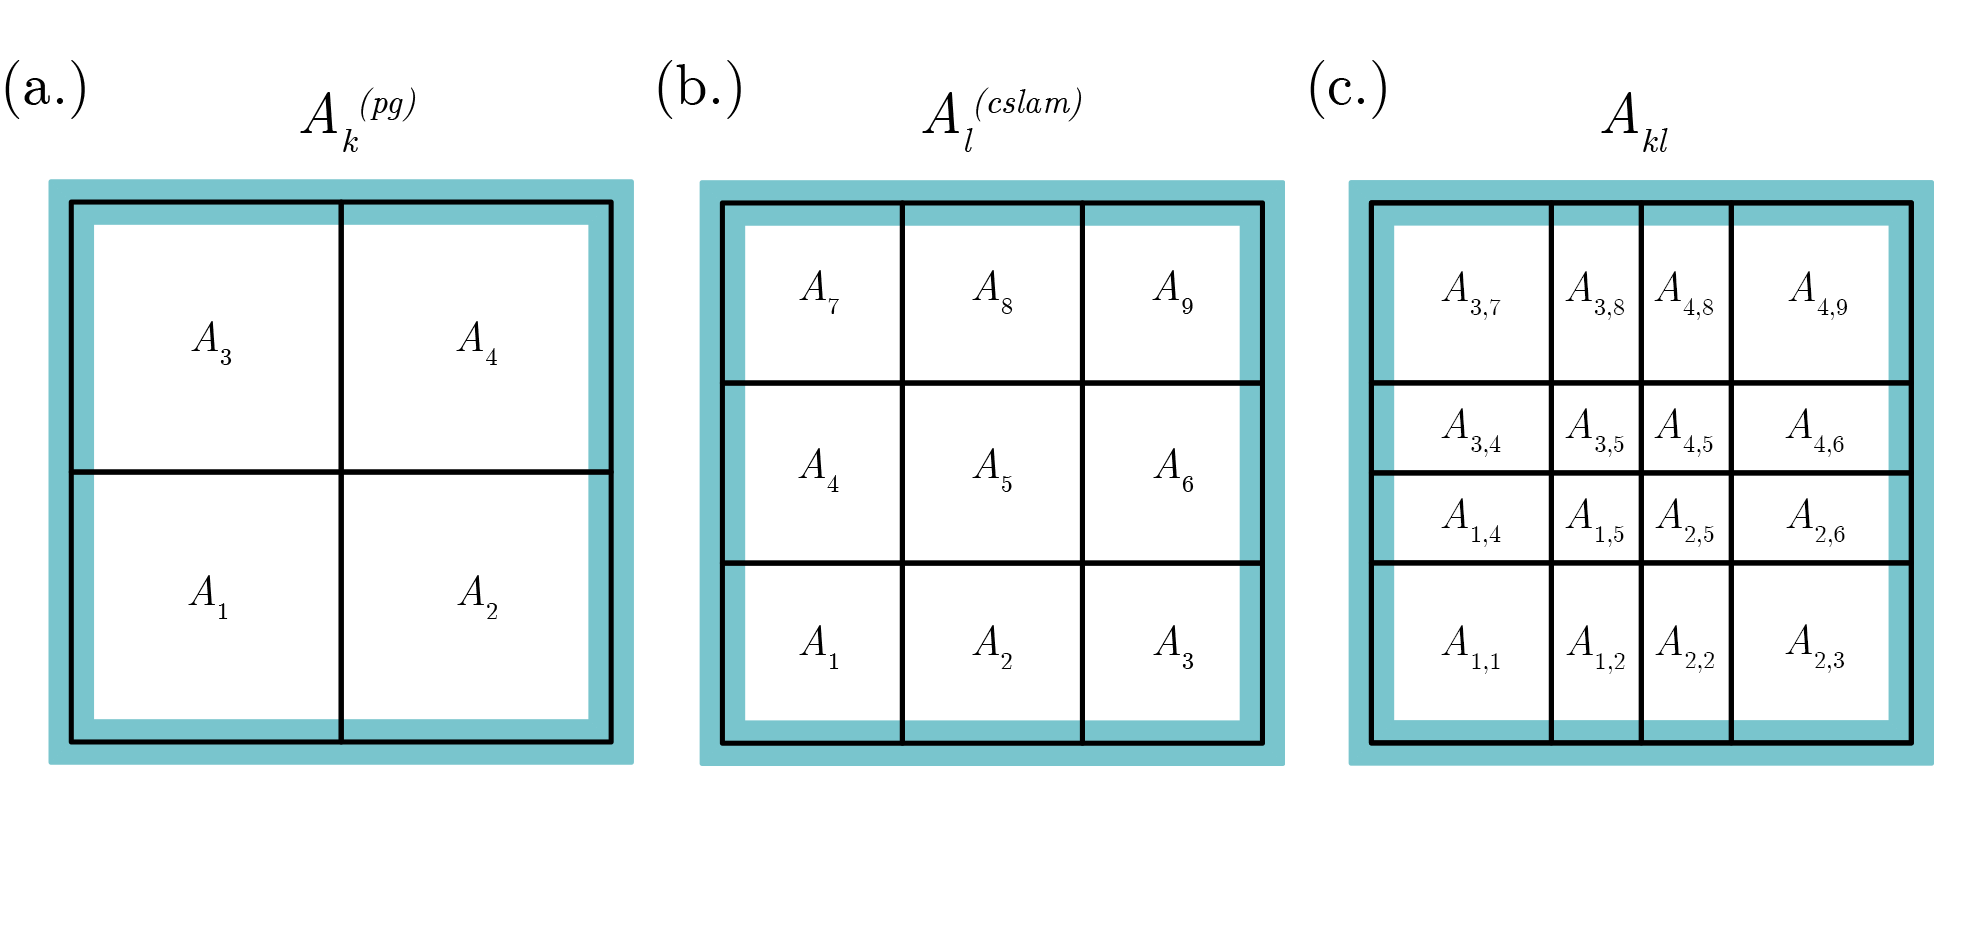
\includegraphics[width=30pc,angle=0]{figs/area-schematic.png}\\
\end{center}
\caption{Indices notation for (a) the $pg2$ grid, (b) the $pg3$ grid and (c) their exchange grid.}
\label{fig:area-schematic}
\end{figure}

Denote the known cell averaged values of dry pressure-level thickness and mixing ratio $\overline{\Delta p}^{(pg3)}$ and $\overline{m}^{(pg3)}$, respectively. We consider a particular layer and for simplicity drop the layer subscript. The same procedure is applied to each layer in a column. The unknowns we would like to compute is the cell-averaged values of the same quantities on the physics grid; $\overline{\Delta p}^{(pg2)}$ and $\overline{m}^{(pg2)}$, respectively. The dry pressure level thickness integrated over the $k$'th physics grid cell is given by
\begin{equation}
\label{eq:p}
\overline{\Delta p}^{(pg2)}_k=\frac{1}{\Delta A^{(pg2)}_k}\sum_{\ell=1}^{nc^2}\left<\delta p\right>_{k\ell},
\end{equation}
where $\left< \delta p\right>_{k\ell}$ is the dry mass in a layer over overlap area $A_{k\ell}$. It is computed by integrating a high-order (2D polynomial of degree 2) reconstruction of pressure-level thickness in each CSLAM cell over the overlap area $A_{k\ell}$
\begin{equation}
\label{eq:pg3dp}
\left< \delta p\right>_{k\ell}=\int_{A_{k\ell}}\left[ \sum_{i+j\le 2}{\mathcal{P}}^{(ij)}_\ell x^{i}y^{j}\right] dA.
\end{equation}
The reconstruction coefficients ${\mathcal{P}}^{(ij)}_\ell$ in CSLAM cell $\ell$ are computed from the cell average pressure level thicknesses on the CSLAM grid $\overline{\Delta p}^{(pg3)}$ and the numerical integration over overlap areas is done by line-integrals. The details of that is given in \cite{LNU2010JCP} and not repeated here.

The average tracer mass per unit area on the physics grid is given by
\begin{equation}
\label{eq:mp}
\overline{m\Delta p}^{(pg2)}_k=\frac{1}{\Delta A^{(pg2)}_k}\sum_{\ell=1}^{nc^2}\left< m\delta p\right>_{k\ell},
\end{equation}
where $\left< m\delta p\right>_{k\ell}$ is the tracer mass over $A_{k\ell}$ resulting from integrating a high-order reconstruction of $\Delta p$ and $m$ combined using the approach outlined in Appendix B of \cite{NL2010JCP} over the overlap area $A_{k\ell}$
\begin{equation}
\label{eq:mp2}
\left< m\delta p\right>_{k\ell}=\int_{A_{k\ell}}\left[ \overline{\Delta p}_\ell^{(pg3)}\sum_{i+j\le 2}{\mathcal{M}}^{(ij)}_\ell x^{i}y^{j}+{\overline{m}}_\ell^{(pg3)}\sum_{i+j\le 2}{\widetilde{{\mathcal{P}}}}^{(ij)}_\ell x^{i}y^{j}\right] dA,
\end{equation}
where ${\widetilde{{\mathcal{P}}}}^{(00)}_\ell={\mathcal{P}}^{(00)}_\ell-\overline{\Delta p}^{(pg3)}_\ell$ and ${\widetilde{{\mathcal{P}}}}^{(ij)}_\ell={\mathcal{P}}^{(ij)}_\ell$ for $i,j>0$, and ${\mathcal{M}}^{(ij)}_\ell$ are the reconstruction coefficients for the mixing ratio in CSLAM cell $A^{(pg3)}_\ell$. A shape-preserving limiter is applied to the reconstruction of mixing ratio $m$ \citep{BJ1989} and not $\Delta p$. This way of combining the reconstruction function for $\Delta p$ and $m$ in \eqref{eq:mp2} ensures that a constant mixing ratio is preserved (consistency), tracer mass is conserved, linear-correlations are preserved and tracer shape-preservation is retained. The mixing ratio on the physics grid is then
\begin{equation}
{\overline{m}}^{(pg2)}_k=\frac{\overline{\left( m\Delta p\right)}^{(pg2)}_k}{\overline{\Delta p}^{(pg2)}_k},
\end{equation}
where $\overline{\Delta p}^{(pg2)}_k$ is given in \eqref{eq:p}. 

Perhaps surprisingly a much more challenging problem is to map tracer increments (or state) from the physics grid to the CSLAM grid while retaining important properties such as mass-conservation, consistency, and correlation preservation. Why this mapping problem is challenging is explained in detail in Section \ref{sec:why} after having defined important properties for mapping physics increments/tendencies.
\subsection{Mapping tracer increments from $A^{(pg2)}$ to $A^{(pg3)}$ (physics to CSLAM grid)}\label{sec:pgtonc}
The increments from the parameterizations are computed on the physics grid. The tracer increment in physics grid cell $k$ is denoted $\overline{f}_k^{(pg2)}$ so that the updated mixing ratio on the physics grid is ${\overline{m}}^{(pg2)}_k+\overline{f}_k^{(pg2)}$. The problem is how to map $\overline{f}_k^{(pg2)}$ to the CSLAM control volumes, to obtain ${\overline{f}}^{(pg3)}$, satisfying the following constraints:
\begin{enumerate}
\item {\bf{Local mass-conservation}}: At a minimum total physics mass forcing on an element computed on the physics grid should equal the element physics mass forcing on the CSLAM grid
\begin{equation}
{\overline{f}}_k^{(pg2)}{\overline{\Delta p}}^{(pg2)}_k\Delta A_k^{(pg2)}=\sum_{\ell=1}^{nc^2}\left[{\overline{\Delta p}}^{(pg3)}_\ell {\overline{f}}^{(pg3)}_\ell\Delta A_{k\ell}\right],
\end{equation}
where $\overline{\Delta p}^{(pg2)}_k$ is the pressure level thickness in physics grid cell $k$ and similarly for $\overline{\Delta p}^{(pg3)}$. We enforce a more local constraint in which only mass-increments overlapping with a particular CSLAM cell contributes to the mass-increment in that CSLAM cell.
\item {\bf{Local shape-preservation in mixing ratio}}: The increments mapped to the CSLAM grid and added to the previous CSLAM state should not produce values smaller than the updated physics grid mixing ratios, ${\overline{m}}^{(pg2)}_k+\overline{f}_k^{(pg2)}$, or values smaller than the existing CSLAM mixing ratios that overlap with physics grid cell $A_\ell$
\begin{equation}
\label{eq:min}
\overline{m}^{(pg3)}_\ell+{\overline{f}}^{(pg3)}_\ell \ge \overline{m}^{(min)}_k=\min \left( {\overline{m}}^{(pg2)}_k+{\overline{f}}_k^{(pg2)},\left\{ {\overline{m}}_{k\ell} |\ell=1,nc^2\right\} \right),
\end{equation}
where
\begin{equation}
\label{eq:moverlap2}
\overline{m}_{k\ell}=\frac{\left< m\delta p_{k\ell}\right> }{\left< \delta p_{k\ell}\right>}.
\end{equation}
The nominator and denominator in \eqref{eq:moverlap2} are defined in \eqref{eq:pg3dp} and \eqref{eq:mp2}, respectively. In particular this means that an increment, when mapped to the $pg3$ grid, should not drive the state negative (described in detail below as the `negativity' problem).

A similar definition apply for maxima
\begin{equation}
\label{eq:max}
{\overline{m}}^{(pg3)}_\ell+{\overline{f}}^{(pg3)}_\ell \le \overline{m}_k^{(max)}=\max \left( {\overline{m}}^{(pg2)}_k+\overline{f}_k^{(pg2)},\left\{ {\overline{m}}_{k\ell} |\ell=1,nc^2\right\} \right),
\end{equation}
\item {\bf{Linear correlation preservation}}: The physics forcing must not disrupt linear tracer correlation between species on the CSLAM grid \citep[see, e.g., ][]{LT2011QJR}, i.e. if two tracers are linearly correlated and the physics increment preserves linear correlations on the physics grid then the tracer increment on the CSLAM grid must not disrupt linear correlations.
\item {\bf{Consistency}}: A non-zero constant mixing ratio increment from physics, $cnst$, on the physics grid, $\overline{f}_k^{(pg2)}=cnst$ $\forall k$, must result in the same (constant) forcing on the CSLAM grid, $\overline{f}_\ell^{(pg3)}=\overline{f}_k^{(pg2)}=cnst$ $\forall \ell$.
\end{enumerate}
To motivate the algorithm that will simultaneously satisfy 1-4 it is informative to discuss how `standard' mapping algorithms will violate one or more of the constraints:
\subsubsection{Why `conventional' conservative remapping will not work}\label{sec:why}
It is helpful to analyze in detail why conventional remapping can not satisfy properties 1-4 above. Assume that one remaps the mass-increments in exactly the same way as the mapping of mixing ratio state from the CSLAM grid to the physics grid described in section \ref{sec:nctopg}. That is, replace $m$ with $f$ and map from physics grid to the CSLAM grid instead of the other way around. Denote the mapped mass-increment $\widetilde{\overline{f\Delta p}}^{(pg3)}$ and due to the properties of the mapping algorithm the mass-increment is conserved, linear correlation between mass-increments are conserved and shape in mass-increment is preserved. The problems arise when converting from mass to mixing ratio.
\paragraph{Conserve mass but not consistency} 
If ones uses the known pressure-level thickness on the CSLAM grid ${\overline{\Delta p}}^{(pg3)}_k$ to convert from mass-increment to mixing-ratio increment
\begin{equation}
\label{eq:convert1}
\overline{m}^{(pg3)}_k=\frac{\widetilde{\overline{f\Delta p}}^{(pg3)}_k}{{\overline{\Delta p}}^{(pg3)}_k},
\end{equation}
a constant mixing ratio increment is not conserved. Basically the constant increment mapped to the CSLAM grid and converted to mixing ratio increment through \eqref{eq:convert1} will, rather than being constant, reflect the spurious discrepancy between $\widetilde{\overline{\Delta p}}^{(pg3)}_k$ and ${\overline{\Delta p}}^{(pg3)}_k$, where $\widetilde{\overline{\Delta p}}^{(pg3)}_k$ is the pressure-level thickness mapped from the $pg2$ grid to the $pg3$ grid. That said, mass will be conserved since the dynamical core state has ${\overline{\Delta p}}^{(pg3)}_k$ (unless the increment drives the mixing ratio negative - described in detail below). 
\paragraph{Consistent but not mass-conserving} 
Rather than converting to mixing ratio using ${\overline{\Delta p}}^{(pg3)}_k$, a constant increment can be preserved by using
\begin{equation}
\overline{m}^{(pg3)}_k=\frac{\widetilde{\overline{f\Delta p}}^{(pg3)}_k}{\widetilde{\overline{\Delta p}}^{(pg3)}_k},
\end{equation}
instead. But now mass-conservation is lost since, again, $\widetilde{\overline{\Delta p}}^{(pg2)}_k\ne {\overline{\Delta p}}^{(pg2)}_k$. This issue is similar to the mass-wind inconsistency found in specified dynamics applications \citep[e.g.][]{JKLSBCRE2001QJR,L2009LNCE}. 

\begin{figure}[t]
\begin{center}
\noindent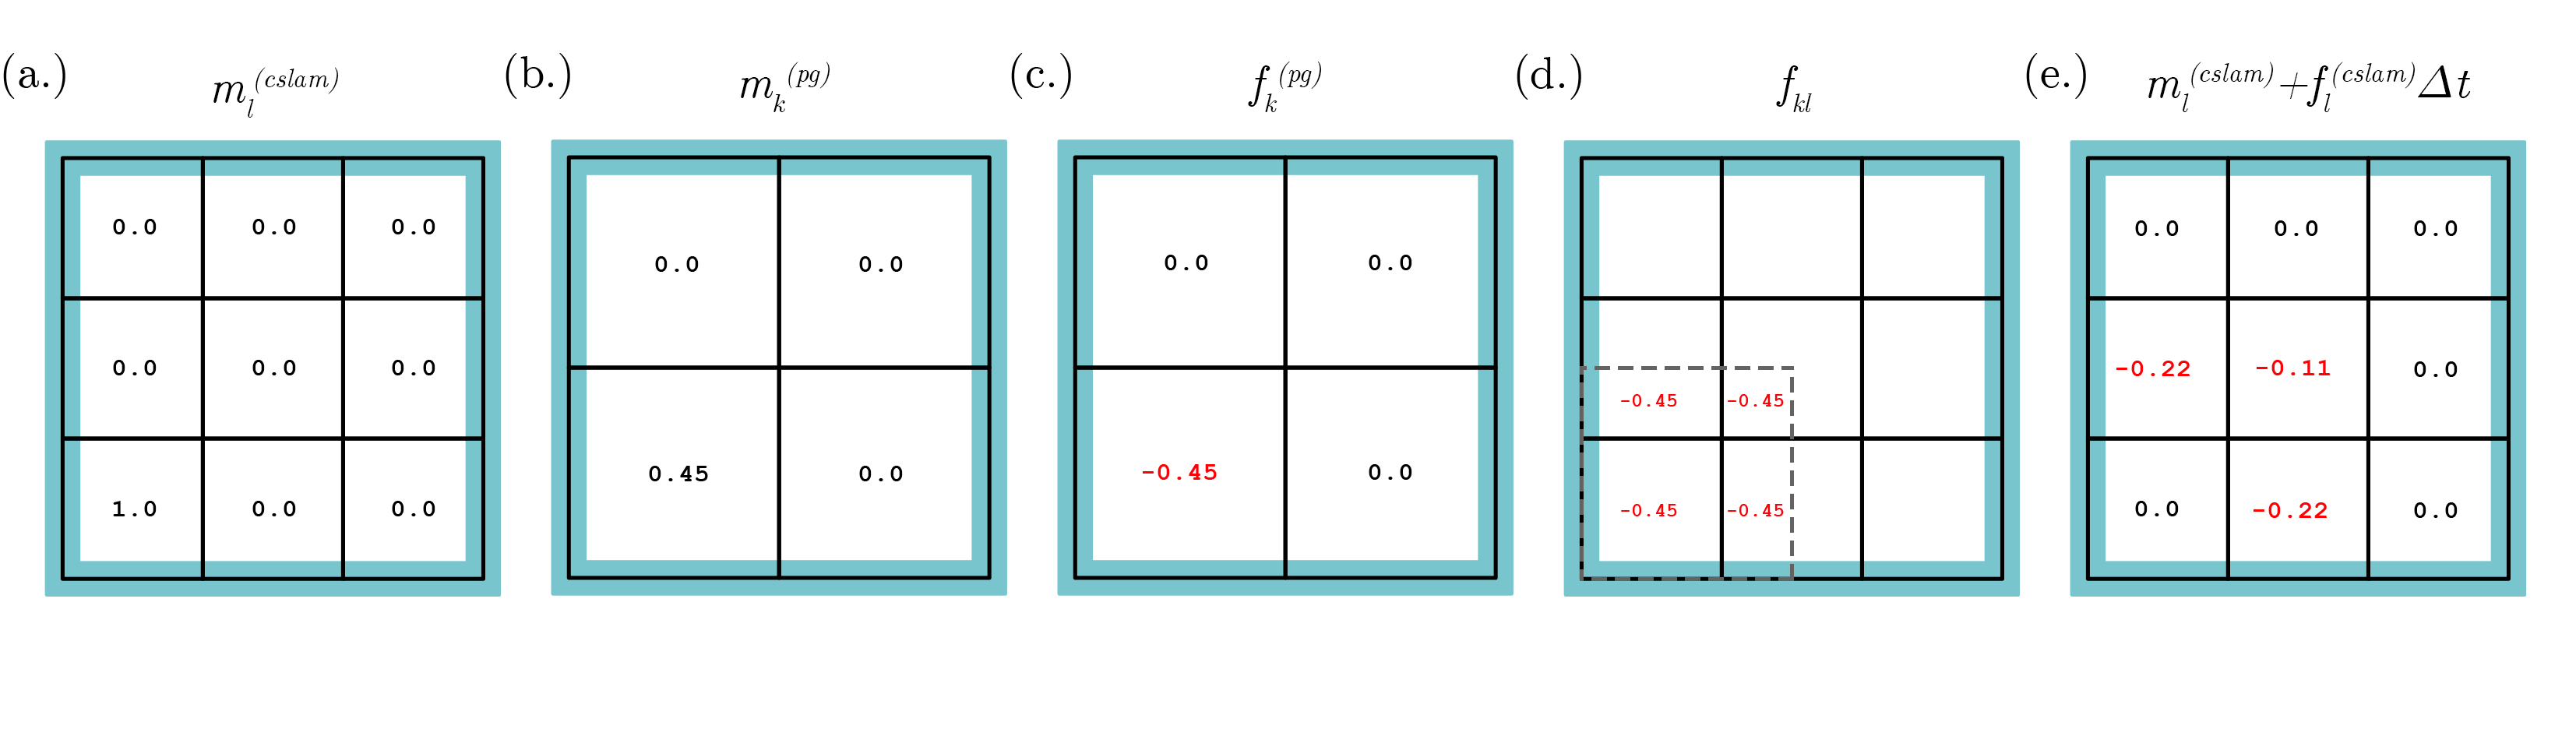
\includegraphics[width=30pc,angle=0]{figs/alg-schematic.png}\\
\end{center}
\caption{Schematic illustration of the `negativity problem' in a single element. (a.) Initial CSLAM tracer values, (b.) mapped to $pg2$, (c) produces a tracer increment on $pg2$, (d.) with negative increments on the exchange grid overlying CSLAM cells in (a) that were initially zero and (e) driving those mixing ratios negative.}
\label{fig:alg-schematic}
\end{figure}
\paragraph{The `negativity' problem and linear correlations} 
Even if one could derive a reversible map for mapping ${\overline{\Delta p}}^{(pg2)}$ from the physics grid to the CSLAM grid, there could still be problems if the increment drives the mixing ratios negative (or overshooting occurs) on the CSLAM grid. This can easily happen for tracers, such as cloud liquid amount and cloud ice amount, that are zero in most of the domain and non-zero in localized areas/points (where there are clouds). We refer to this as the `negativity problem'. This problem is depicted schematically in Figure~\ref{fig:alg-schematic}. Consider a single element of CSLAM control volumes, containing only a single cell with mixing ratio $1.0$, and $0.0$ everywhere else ($\overline{m}^{(pg3)}_\ell$; Figure ~\ref{fig:alg-schematic}a). The mixing ratios are mapped to the $pg2$ grid using, for simplicity, the piecewise constant method where a constant value inside the $pg2$ cells is used during the integration over overlap cells ($\overline{m}^{(pg2)}_k$; Figure~\ref{fig:alg-schematic}b). Now consider the case in which physics removes all the mass from the physics cell $k$: $\overline{f}^{(pg2)}_k=-\overline{m}^{(pg2)}_k$ (Figure~\ref{fig:alg-schematic}c). The tracer increment is mapped from $pg2$ to $pg3$ using the piecewise constant method. Some of the non-zero increments are now in overlap areas where the original CSLAM grid cells have mixing ratio zero ($\overline{f}_{k\ell}$; Figure~\ref{fig:alg-schematic}d), and hence, the state is driven negative when adding the overlap increment to the CSLAM state (Figure~\ref{fig:alg-schematic}e).  This is referred to as the negativity problem although it can also happen for maxima.

The negativity issue could be avoided if one remaps the physics updated state instead of mapping increments/tendencies. In that case a shape-preserving filter will make sure that the state on the CSLAM grid is not negative (and does not overshoot). That said, if physics does not change the state and it is mapped back to the CSLAM grid then spurious tendencies (proportional to the errors introduced by mapping state from the CSLAM grid to the physics grid and back again) are introduced. Hence it is advantageous to map increments/tendencies since any reasonable algorithm will preserve a zero function.

%In the $pg2$ configuration, mapping the fields to and from the quadrature grid and $pg2$ grid is identical to that described in H18. As discussed above above, in mapping to the physics grid, CAM-SE's Lagrange basis functions are integrated over the $pg2$ control volumes to provide the physics with a volume averaged state. The procedure is accurate to machine precision, conserves thermal energy and dry air mass, and is consistent (i.e., the mapping preserves a constant). The reverse mapping, from the physics grid to the quadrature grid, is done using a tensor-product Lagrange interpolation (see Appendix A in H18). The Lagrange interpolation is consistent, conserves dry air mass ({\color{red}{Peter, is this true?}}), but does not conserve thermal energy. Errors arising from the lack of energy conservation were estimated to be small; about two orders of magnitude less than the energy dissipation due to the dynamical core alone.

%The semi-Lagrangian advection of tracers in our $pg2$ configuration is solved on the CSLAM grid. 





%Interpolation: Traditional Lagrange interpolate of the mixing ratio increment would preserve a constant and could be made shape-preserving using {\em{ad hoc}} filters \citep[e.g.][]{BC2002MWR} but will not inherently preserve mass increment and suffers from the `negativity problem' described above.

As illustrated above a standard remapping method will NOT simultaneously satisfy 1-4 and hence a new algorithm has been derived.
\subsection{New tendency mapping algorithm}\label{sec:massfix}
Although this algorithm is explained and examined for a $pg2$ grid, it is general for any $pgX$ resolution. The problem is how to map the mass-increment on the physics grid, ${\overline{f}}^{(pg2)}\Delta A^{(pg2)}$, to the CSLAM cells that overlap with $\Delta A^{(pg2)}$. To maintain shape-preservation, linear correlations and to avoid the negativity problem locally, it is advantageous to define a mass excess function on the exchange grid $\Delta m_{k\ell}^{(excess)}$. It is basically the maximum amount of mixing ratio that can be removed (in the case ${\overline{f}}^{(pg2)}<0$) without producing new minima in the exchange grid mixing ratio $m_{k\ell}$
\begin{equation}
\Delta m^{(excess)}_{k\ell}=\overline{m}_{k\ell}-\overline{m}_k^{(min)},
\end{equation}
where $\overline{m}_{k\ell}$ is defined in \eqref{eq:moverlap2}. So the maximum amount of mass that we can be removed from the exchange grid cells that span physics grid cell $A_k$ without violating the shape-preservation constraint (\eqref{eq:min} and \eqref{eq:max}) is
\begin{equation}
\sum_\ell \Delta m^{(excess)}_{k\ell}\overline{\Delta p}_{k\ell} \delta A_{k\ell}.
\end{equation}
If physics is designed not to remove more mass than available in $A_k$ (which should be the case for a carefully designed physics package) then it is guaranteed that
\begin{equation}
\label{eq:well-posed}
\sum_\ell \Delta m^{(excess)}_{k\ell}\overline{\Delta p}_{k\ell} \delta A_{k\ell}\ge {\overline{f}}^{(pg2)}\Delta p_k\Delta A^{(pg2)}.
\end{equation}
We distribute the physics mass-forcing (assuming ${\overline{f}}^{(pg2)}<0$) according to the mass excess in each overlap area by solving this equation for $\gamma_k$
\begin{equation}
\label{eq:mass-excess}
\Delta A_k^{(pg2)}\overline{\Delta p}_k^{(pg2)}{\overline{f}}^{(pg2)}=\gamma_k \sum_\ell \Delta m^{(excess)}_{k\ell}\overline{\Delta p}_{k\ell} \delta A_{k\ell},
\end{equation}
and add mass increment (which in this case is negative)
\begin{equation}
\label{eq:mass-incr}
\gamma_k \Delta m^{(excess)}_{k\ell}\overline{\Delta p}_{k\ell} \delta A_{k\ell},
\end{equation}
to the $\ell$th CSLAM cell state ${\overline{m}}^{(pg3)} \overline{\Delta p}^{(pg3)}_\ell \Delta A^{(pg3)}_\ell$. This process is repeated for all physics cells. Note that this problem is a well-posed, i.e. $\gamma_k>0$, since physics will not remove more mass than is locally available \eqref{eq:well-posed}. The way in which the mass-forcing is distributed to the CSLAM cells using the excess function insures that the negativity problem is avoided. Mass is conserved by design and shape-preservation is obtained by using the excess function.

If the physics increment is positive (assuming ${\overline{f}}^{(pg2)}>0$) we define a `lack' function
\begin{equation}
\Delta m^{(lack)}_{k\ell}=\overline{m}_{k\ell}-\overline{m}^{(max)},
\end{equation}
and solve
\begin{equation}
\label{eq:mass-lack}
\overline{\Delta p}_k^{(pg2)}{\overline{f}}^{(pg2)}\Delta A_k^{(pg2)}=\gamma_k \sum_\ell \left[ \Delta m^{(lack)}_{k\ell}\overline{\Delta p}_{k\ell} \delta A_{k\ell}\right],
\end{equation}
for $\gamma_k$ and follow the same procedure as for mass excess. Since positive and negative forcing is treated in exactly the same way, linear correlations are preserved. Note how the definition of the excess/lack function insures linear correlation preservation; for example, if one would prevent negative values and not do anything about overshoots then linear correlations would not be preserved since the minima and maxima are not treated in the same way.

While the above algorithm satisfies properties 1-4 in section \ref{sec:pgtonc}, it is not a high-order algorithm in terms of formal accuracy. This is illustrated in Figure \ref{fig:mapping} (row 3) where a smooth analytical tendency \citep[approximate spherical harmonic of order 32 and azimuthal wave number 16; ][]{J1999MWR}
\begin{equation}
\label{eq:Y32}
f^{(pg2)}=\frac{1}{2}+\frac{1}{2}\cos(16\lambda)\sin(2\theta)^{16},
\end{equation}
where $(\lambda,\theta)$ is latitude-longitude, is mapped from $pg2$ to $pg3$ grid using this algorithm assuming $m^{(pg3)}_\ell=0, \quad \forall \ell$. The errors in the mapping are not always aligned with large gradients in the analytical function as would be expected for a `traditional' interpolation algorithm. The errors are maximum on the order of 60$\%$. To reduce errors we therefore perform a higher-order pre-allocation of tendencies that is not mass-conserving but satisfies properties 2,3, and 4 in Section \ref{sec:pgtonc}.

\begin{figure}[t]
\begin{center}
\noindent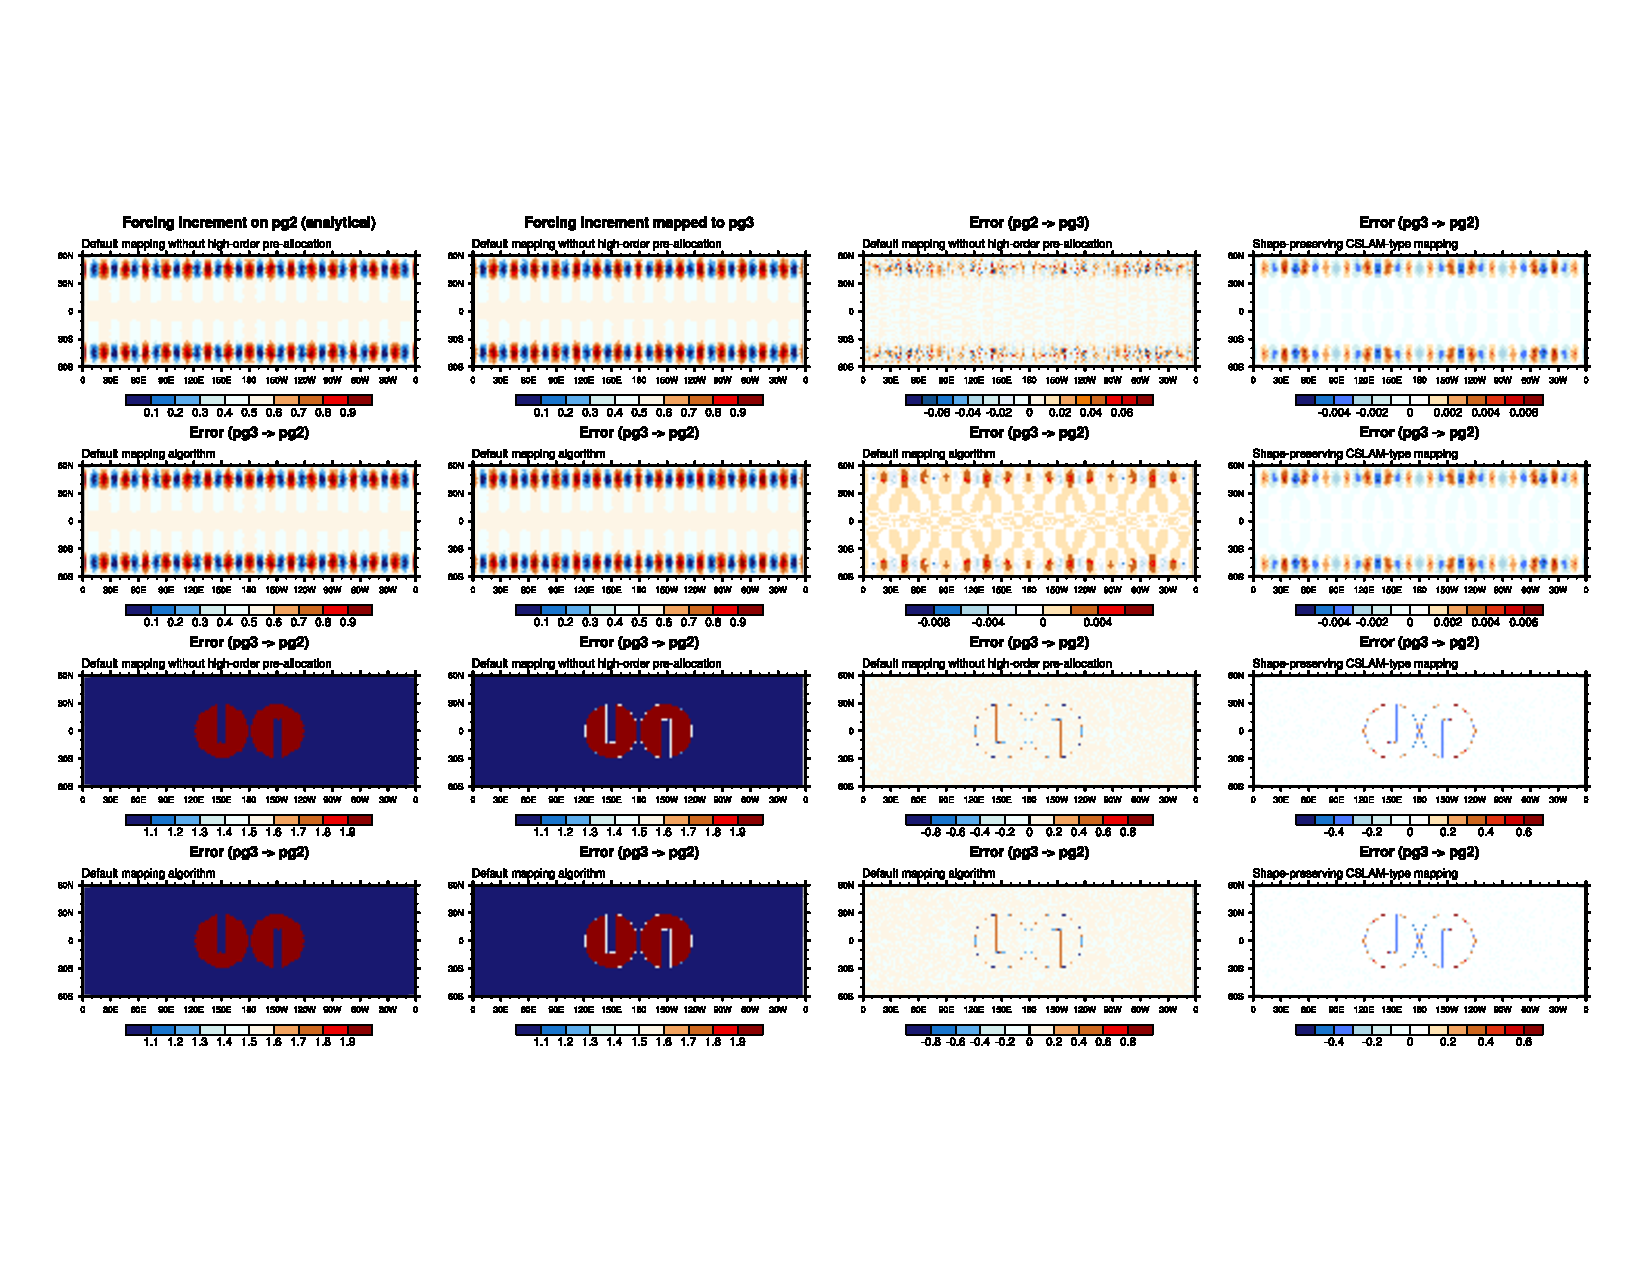
\includegraphics[width=30pc,angle=0]{figs/mapping.pdf}\\
\end{center}
\caption{Mapping of idealized functions from $pg2$ (column 1) to $pg3$ (columns 2) and errors (column 3) using the new tendency algorithm only (row 1 and 3) and new tendency algorithm with the high-order pre-allocation (row 2 and 4). Column 4 shows the errors in mapping the same distributions from  $pg3$ to $pg2$ using traditional remapping (CSLAM technology).}
\label{fig:mapping}
\end{figure}

%Similarly we define a mass lack function

%which is the maximum amount of mixing ratio that can be added without creating new maxima.

\subsection{High-order (non-conservative) pre-allocation of tracer tendencies}
A high-order tracer mass increment in overlap area $A_{k\ell}$ can be computed using the following formula
\begin{equation}
\label{eq:mp3}
\left< f\delta p\right>_{k\ell}=\int_{A_{k\ell}}\left[ \overline{\Delta p}_\ell^{(pg3)}\sum_{i+j\le 2}{\mathcal{F}}^{(ij)}_k x^{i}y^{j}+{\overline{f}}_k^{(pg2)}\sum_{i+j\le 2}{\widetilde{{\mathcal{P}}}}^{(ij)}_\ell x^{i}y^{j}\right] dA,
\end{equation}
where $\mathcal{F}^{(ij)}_k$ is the forcing increment reconstruction coefficients in the $k$th physics grid cell and ${\overline{f}}_k^{(pg2)}$ is the average physics increment in the $k$th physics grid cell. Note that we are using the known dry pressure reconstruction coefficients on the $pg3$ grid instead of reconstructing sub-grid-scale pressure variations from the physics grid cell averaged values. We can do that since the dry pressure is not modified by physics. This highlights the importance of a dry-pressure formulation of the dynamical core when separating physics and dynamics grids \citep{LetAl2018JAMES}. If the physics forcing is constant then $\left< f\delta p\right>_{k\ell}$ exactly equals $\left<\delta p\right>_{k\ell}$ from \eqref{eq:pg3dp}; in other words, the mapping is designed to be reversible in dry pressure. The physics increment in terms of mixing ratio change is given by
\begin{equation}
\label{eq:pg3fq}
\overline{f}_{k\ell}=\frac{\left< f\delta p\right>_{k\ell}}{\left<\delta p\right>_{k\ell}},
\end{equation}
where the denominator is given by \eqref{eq:pg3dp}.

Shape-preservation, as defined by \eqref{eq:min} and \eqref{eq:max}, is enforced by eliminating under and overshoots on the exchange grid by modifying the forcing increment $\overline{f}_{k\ell}$ so that shape-preservation is not violated in the overlap areas{\footnote{In the computation of $\overline{m}_{k\ell}$ there can be small overshoots and undershoots (due to numerical integration errors) compared to the CSLAM cell average values $\overline{m}^{(pg3)}_\ell$ that it overlaps with so we set
\begin{equation}
\overline{m}_k^{(min)}=\min \left( \overline{m}_k^{(min)},\left\{ \overline{m}^{(pg)}_\ell)|\ell=1,nc^2\right\} \right)
\end{equation}}}
\begin{equation}
\overline{m}_k^{(min)} \le \overline{m}_{k\ell}+\widetilde{\overline{f}}_{k\ell} \le \overline{m}_k^{(max)}.
\end{equation}
While this algorithm preserves linear correlations, shape, and is consistent, is it not mass-conservative. Hence the remaining physics increment not allocated in the algorithm above is allocated using the new tendency algorithm described in Section \ref{sec:massfix}.

Combining the high-order pre-allocation algorithm with the new tendency algorithm (which in this case can also be considered as a mass-fixer that does not disrupt correlation-preservation, shape and consistency) leads to an order-of-magnitude reduction in mapping errors for a smooth function (see Figure \ref{fig:mapping} row 3 and 4) while full-filling the mass-conservation, shape-preservation, linear correlation and consistency  constraint. Mass and linear correlation preservation is illustrated in the baroclinic wave test with terminator chemistry test in Section \ref{sec:fkessler}. Shape-preservation and consistency is demonstrated in an idealized mapping test where a smooth function, see \eqref{eq:Y32}, and a slotted-cylinder \citep[see equation 12 in ][]{LSPT2012GMD} are mapped to/from the $pg2$ and $pg3$ grids. Since the background value in the mapping of the slotted-cylinder field is preserved the mapping algorithm is consistent. Since no new over- and undershoots are produced (particularly obvious in the mapping of the slotted cylinders) the mapping is shape-preserving. We also note that the mapping errors with the default algorithm (higher-order pre-allocation with new tendency algorithm) are similar to the errors in mapping the same field from $pg3$ to $pg2$ using traditional remapping with CSLAM technology (column 4 in Figure \ref{fig:mapping}).


%A high-order estimate of the physics increment in the $A_{k\ell}$th overlap cell, that is not mass-conserving, can be computed as
%\begin{equation}
%\label{eq:mp3}
%\overline{f}_{k\ell}=\frac{1}{\delta A_{k\ell}}\int_{A_{k\ell}}\left[ \sum_{i+j\le 2}{\mathcal{F}}^{(ij)}_k x^{i}y^{j}\right] dA,
%\end{equation}
%where $\mathcal{F}^{(ij)}_k$ are the recontruction coefficients for the physics increment $f$ in the $k$th physics grid cell. For reasons that will become clear a shape-preserving limiter is not applied when computing $\mathcal{F}^{(ij)}_k$. Each overlap increment is added to the CSLAM opverlap state $\overline{m}_{k\ell}$ 
%\begin{equation}
%\overline{m}_{k\ell}+\tilde{\overline{f}}_{k\ell},
%\end{equation}
%where $\tilde{\overline{f}}_{k\ell}$ is $\overline{f}_{k\ell}$ `cropped' so that shape-preservation is not violated locally

{\color{red}Describe algorithm here}

{\color{red}Peter -  I think the results of the terminator tests should be mentioned here. We could just put in a sentence saying it passes. But I'm assuming that if we don't use the algorithm that weights the tendency by the amount of available mixing ratio, it will fail. If that's the case, we could just do a two panel plot showing the iCLy at day 15 for with and without the algorithm.}

\subsection{Model Configurations}\label{sec:config}

Two model configurations using the Community Earth System Model, version 2.1 (CESM2.1; \url{https://doi.org/10.5065/D67H1H0V}) are chosen to carry out the objectives discussed in Section~\ref{sec:intro}. To test the hypothesis, that the $pg2$ grid reduces spurious grid-noise over mountainous regions, a Held-Suarez configuration \citep[$FHS94$ compset;][]{HS1994} modified to include real world topography is analyzed. H18 indicate that this configuration tends to have more grid-noise over steep terrain than in a more complex configuration using CAM, version 6 moist physics \citep[CAM6;][]{}, and is therefore a conservative choice for evaluating any change in grid imprinting between $pg3$ and $pg2$. 

To understand whether the resolved scales of motion are influenced by a coarser resolution physics grid, a suite of aqua-planet simulations \citep{NH2000ASL,MWO2016JAMES} are carried out over a range of spectral-element grid resolutions, using CAM6 physics ($QPC6$ compset). The aqua-planet is an ocean covered planet in perpetual equinox, with fixed, zonally-symmetric sea surface temperatures idealized after present day Earth \citep[$QOBS$ in][]{NH2000ASL}. While the dynamics time-step, $\Delta t_{dyn}$, varies with resolution according to a CFL criterion, there is no established standard for how the physics time-step, $\Delta t_{phys}$, should vary across resolutions. This is further complicated by several studies indicating a high sensitivity of solutions to $\Delta t_{phys}$ in CAM  \citep{WO2003QJR,W2013QJRMS,WETAL2015JAMES,HR2018JAMES}.

Here, a scaling for $\Delta t_{phys}$ across resolutions is proposed, based on results of the moist bubble test \citep{HR2018JAMES} using CAM-SE-CSLAM and detailed in Appendix~\ref{sec:app1}. The basis for the scaling is to alleviate truncation errors that arise in the moist bubble test when $\Delta t_{phys}$ is too large. The scaling is linear in grid-spacing,
\begin{equation}
\Delta t_{phys} = \Delta t_{phys,0} \times \frac{N_e}{N_{e,0}}~s,\label{eq:dt-scale}
\end{equation}
where $\Delta t_{phys,0}$ is taken to be the standard $1800 s$ used in CAM-SE-CSLAM at low resolution, $N_{e,0} = 30$ (equivalent to a dynamics grid-spacing of $111.2km$). $N_e$ refers to the horizontal resolution of the grid; each of the six panels of the cubed-sphere are divided into $N_e \times N_e$ elements. Throughout the paper, spectral-element grid resolutions are denoted by an $ne$ followed by the quantity $N_e$, e.g., $ne30$.

The only other parameter varied across resolutions modulates the strength of explicit numerical dissipation. The spectral element method is not implicitly diffusive, so fourth-order hyper-viscosity operators are applied to the state to suppress numerical artifacts. The scaling of the hyper-viscosity coefficients, $\nu$, across resolutions is defined as,
\begin{align}
\nu_T = \nu_{vor} &= 0.30\times \left(\frac{30}{N_e}1.1\times 10^5\right)^3\, \frac{m^4}{s}, \\
\nu_p = \nu_{div} &= 0.751\times \left(\frac{30}{N_e}1.1\times 10^5\right)^3\, \frac{m^4}{s},
\label{eq:hypervis}
\end{align}
where subscripts $T,~vor,~p,~div$ refer to state variables the operators are applied to, temperature, vorticity, pressure and divergence, respectively. The scaling reduces the coefficient by an order of magnitude for each doubling of the resolution \citep[as in][]{LetAl2018JAMES}. No explicit dissipation of tracers (e.g., water vapor) is required since the semi-Lagrangian numerics in CSLAM are diffusive.

\section{Results}\label{sec:results}

\subsection{Held-Suarez with Topography}\label{sec:hs94}

Flow over topography can result in significant grid imprinting using the spectral element method \citep[][H18]{gmdd-8-4623-2015}. Figure \ref{fig:fhs-contours} shows the results of the Held-Suarez with topography simulations. The middle panel is the vertical pressure velocity, $\omega$, averaged over two years, over the Andes and Himalayan region at two different levels in the mid-troposphere, using the $ne30pg3$ grid. The fields are displayed as a raster plot on the physics grid, so that individual extrema, which characterize the flow over the Andes between about $10^\circ-20^\circ$ S, may be identified as spurious. Near the foot of the Himalayas, between about $20^\circ-30^\circ$ N, there are parallel stripes of extrema aligned with the mountain front that appear to be spurious $2\Delta x$ oscillations.

\begin{figure}[t]
\begin{center}
\noindent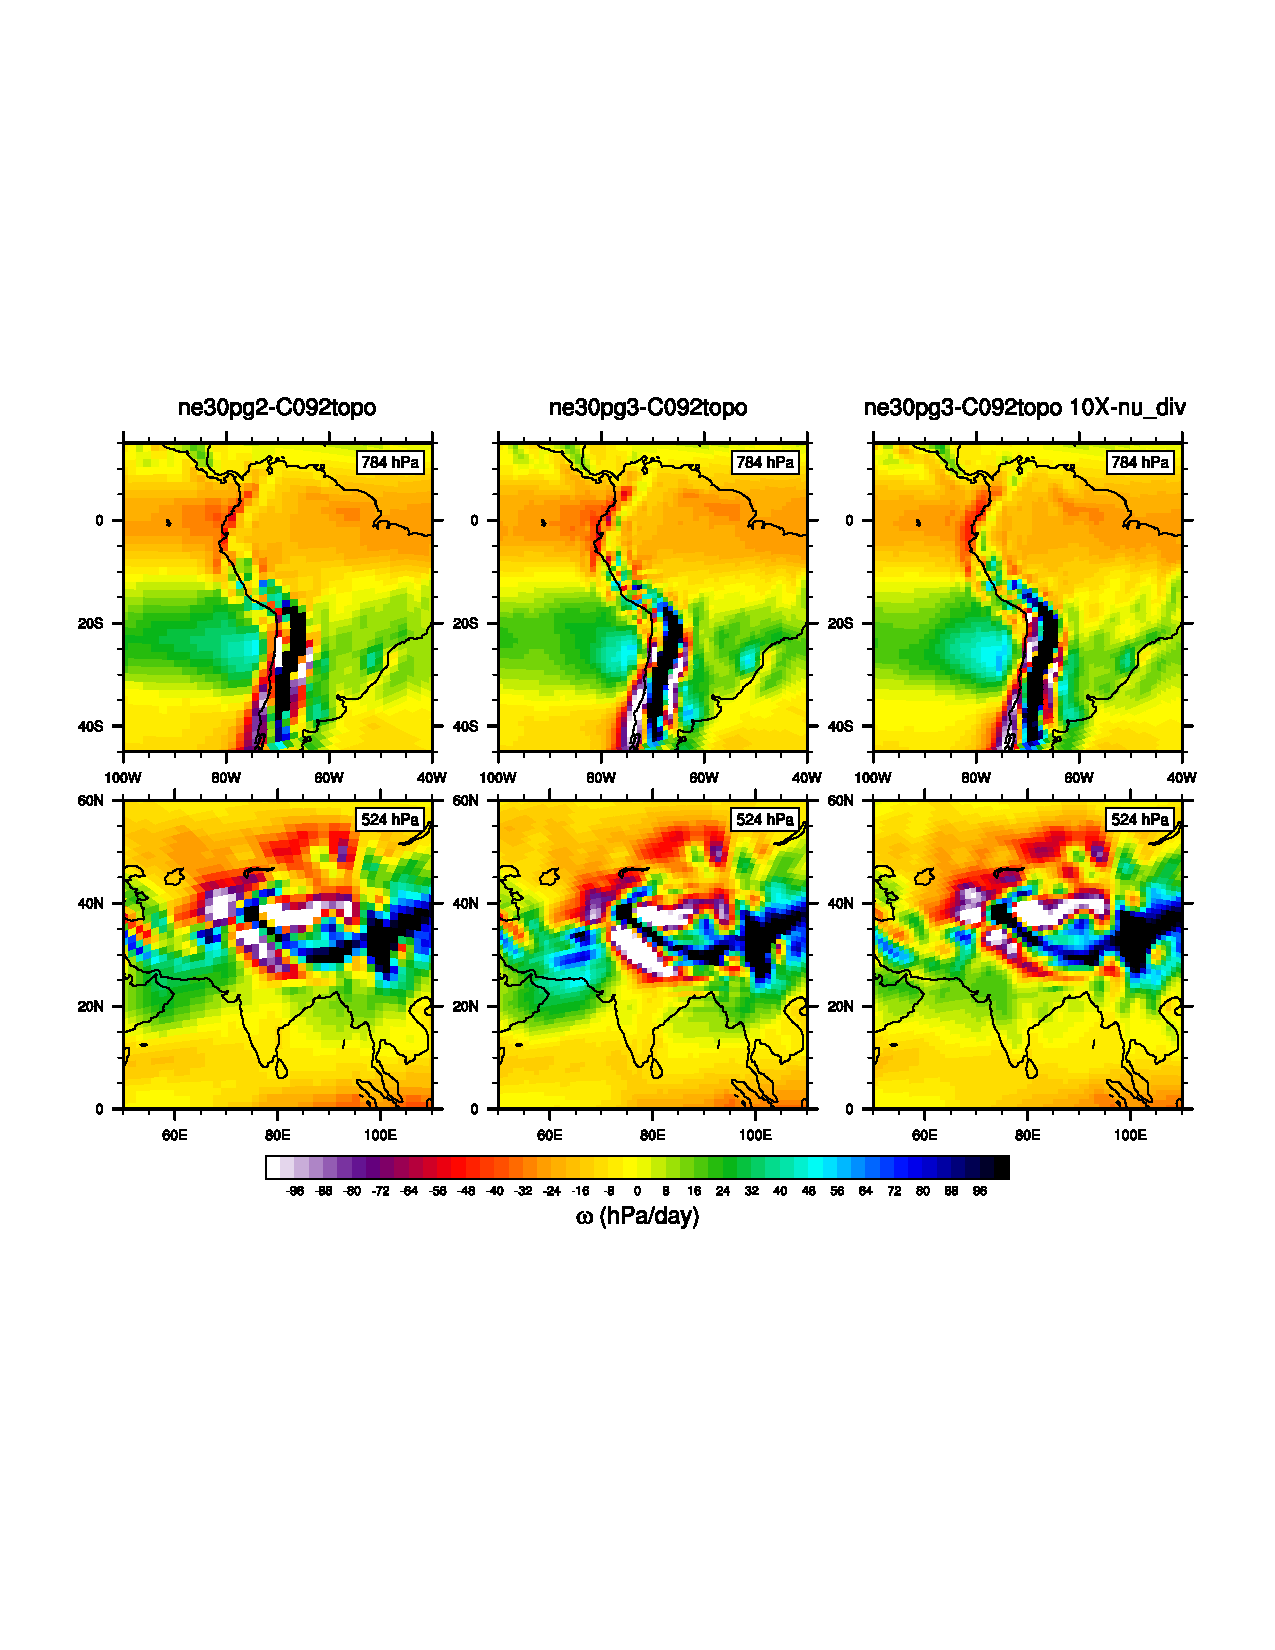
\includegraphics[width=30pc,angle=0]{figs/fhstopo_ne30pg2-v-ne30pg3-v-10Xnudiv.pdf}\\
\end{center}
\caption{Mean $\omega$ at two model levels in the middle troposphere, in a Held-Suarez configuration outfitted with real world topography. (Left) $ne30pg2$ (Middle) $ne30pg3$ and (Right) $ne30pg3$ with the divergence damping coefficient, $\nu_{div}$, increased by an order of magnitude. The $\omega$ fields are computed from a two-year simulation. The data are presented on a raster plot in order to identify individual grid cells}
\label{fig:fhs-contours}
\end{figure}

As discussed in H18, grid imprinting over mountainous terrain tends to occur in regions of weak gravitational stability, causing extrema to extend through the full depth of the troposphere as resolved updrafts and downdrafts. Thus, grid imprinting over mountains may be alleviated through increasing the divergence damping in the model. Figure \ref{fig:fhs-contours} (right panel) repeats the $ne30pg3$ simulation through increasing $\nu_{div}$ by an order of magnitude. The spurious noise over the Andes and the Himalayas are damped, and grid point extrema tend to diffuse into neighboring grid cells. The wavenumber-power spectrum of the kinetic energy due to divergent flow (Figure \ref{fig:fhs-div}) confirms that divergent modes are damped at higher wavenumbers (greater then 30), by about an order of magnitude relative to the default $ne30pg3$ simulation.

\begin{figure}[t]
\begin{center}
\noindent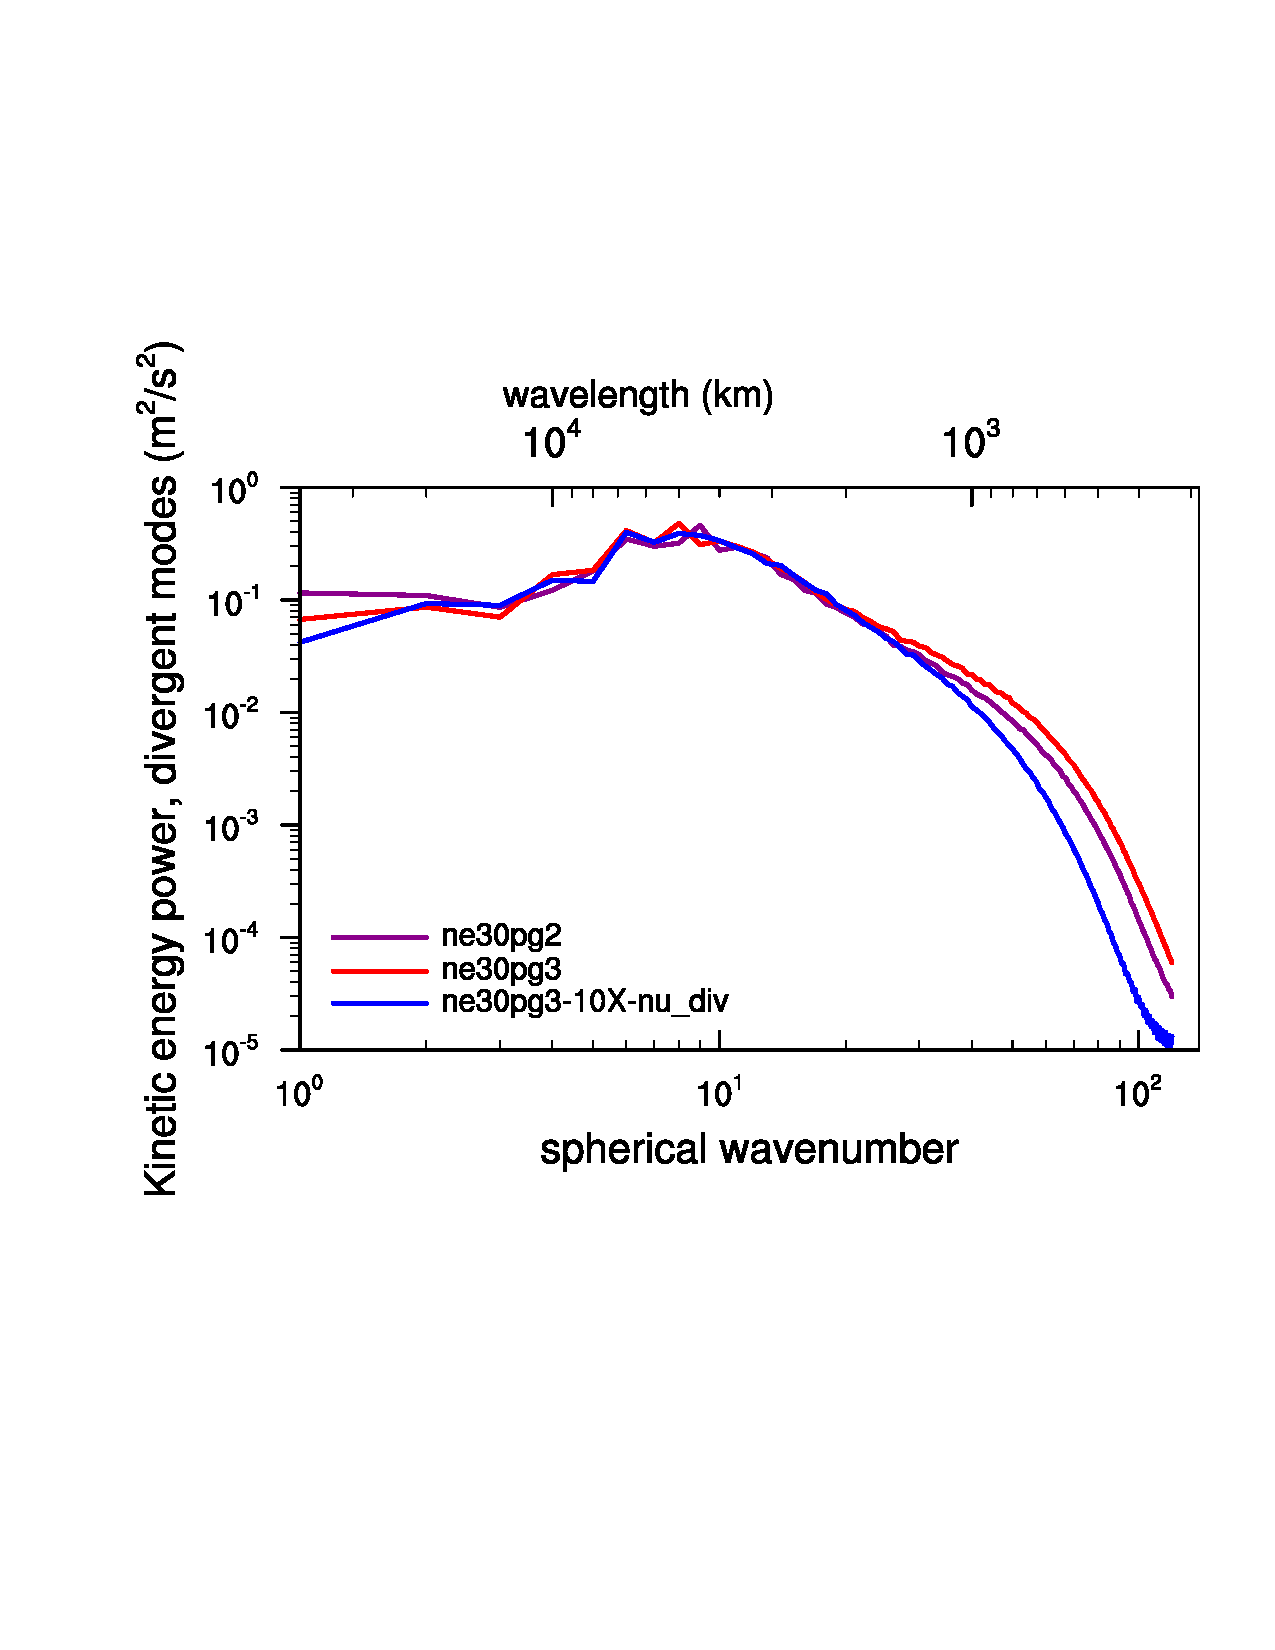
\includegraphics[width=25pc,angle=0]{figs/fhstopo_Divergence_ne30pg2-v-ne30pg3-v-10Xnudiv.pdf}\\
\end{center}
\caption{Kinetic energy power spectrum arising from divergent modes in $ne30pg3$, $ne30pg2$ and $ne30pg3$ with the divergence damping coefficient, $\nu_{div}$, increased by an order of magnitude, in the Held-Suarez with topography simulations. Spectra computed from five months of six-hourly winds.}
\label{fig:fhs-div}
\end{figure}

The $\omega$ field of the $ne30pg2$ simulation is provided in Figure \ref{fig:fhs-contours} (left panel). Grid cell extrema over the Andes is less prevalent than in the $ne30pg3$ simulation, as seen by the reduction in large magnitude $\omega$ (e.g., red grid cells). The spurious oscillations at the foot of the Himalayas appear to have been entirely eliminated. This improvement in grid imprinting is due to the consistent smoothness properties of the control volumes in the $pg2$ grid compared with the $pg3$ grid discussed in Section \ref{sec:intro}, and these results are consistent with our hypothesis. The divergent modes are marginally damped relative to $ne30pg3$ for wavenumbers greater than about 50, but are an order of magnitude larger than in the enhanced divergence damping $ne30pg3$ run (Figure \ref{fig:fhs-div}). From a model development standpoint, the $pg2$ configuration is preferable to placing additional constraints on $\nu_{div}$ in a $pg3$ configuration, since this coefficient is one of only a handful of free parameters available to tune CAM-SE.

\subsection{Aqua-planets}\label{sec:aquaplanet}

The Tropical regions are very sensitive to horizontal resolution, primarily due to the scale dependence of resolved updrafts and downdrafts at hydrostatic scales \citep{HR2017JCLIM,HR2018JAMES}. The vertical velocity of updrafts and downdrafts is related to the horizontal length scales of buoyancy the model is able to support. This can be demonstrated through a scale analysis of the Poisson equation \citep{JR2016QJRMS} valid for hydrostatic scales, showing that the ratio of the scale of $\omega$ at two resolutions, due to their respective buoyancies is,
\begin{equation}
\frac{\omega_{\Delta x_1}}{\omega_{\Delta x_2}} =  \frac{D_{\Delta x_2}}{D_{\Delta x_1}}~,\label{eq:w-scale}
\end{equation}
where $D_{\Delta x}$ is a characteristic buoyancy horizontal length scale for grid-spacing $\Delta x$ (hereafter referred to as the {\em{forcing scale}}), and it is presumed that the magnitude of the buoyancy and the vertical scale of the buoyancy is unchanged or compensating across the two resolutions. Equation~\ref{eq:w-scale} indicates that the magnitude of the vertical velocity scales like the inverse of the forcing scale, which was verified in a simple moist bubble configuration using CAM-SE and the CAM finite-volume dynamical core \citep{HR2018JAMES} and using CAM-SE-CSLAM (Appendix~\ref{sec:app1}). It is by no means trivial that equation~\ref{eq:w-scale} holds for the moist bubble test, since the scaling is derived from the dry anelastic equations.

In aqua-planet simulations using CAM-SE, the forcing scale is grid-limited, varying with resolution in the range of five to ten times the grid-spacing \citep{HR2018JAMES}. From equation~\ref{eq:w-scale}, this grid-dependence explains why the updrafts and downdrafts are so sensitive to horizontal resolution. A grid-limited forcing scale is analogous to an effective resolution, which is the characteristic length scale below which the solution becomes contaminated by numerical artifacts, and the features are overly damped due to numerical dissipation. The effective resolution may be inferred from kinetic energy spectra as the wavenumber where the slope of the spectrum becomes steeper than the observationally determined slope \citep{S2011LNCSE}. In the CESM2 release of CAM-SE, this criterion occurs near wavenumber 60 \citep[see Figure 6 in][]{LetAl2018JAMES}, a length scale of about six times the grid spacing and overlapping with the estimated forcing scale.

When the physics and dynamics grids are of different resolutions, which grid determines the models characteristic forcing scale? The remainder of section~\ref{sec:results} attempts to address this question using spectral element grids at low resolution (Section~\ref{sec:lores}), high resolution (Section~\ref{sec:hires}) and across all resolutions typical of present day climate models (Section~\ref{sec:allres}).

\subsubsection{Low Resolution}\label{sec:lores}

The question posed above may be addressed through comparing $ne30pg2$, where $\Delta x_{phys} = 166.8km$, $\frac{3}{2}$ times larger than the dynamics grid spacing, $\Delta x_{dyn} = 111.2km$, to a simulation where both are equal to the physics grid spacing, $\Delta x_{dyn} = \Delta x_{phys} = 166.8 km$ ($ne20pg3$), and another simulation where both are equal to the dynamics grid spacing, $\Delta x_{dyn} = \Delta x_{phys} = 111.2 km$ ($ne30pg3$). The resolvable scales in the $ne30pg2$ solution are expected to be bounded by the $ne20pg3$ and $ne30pg3$ solutions. Although according to equation~\ref{eq:dt-scale}, $\Delta t_{phys}$ for $ne20$ grids should be different from $ne30$ grids, here it is set to the $ne30$ value (see Table~\ref{table:grids-lo}) in order to reduce the differences between the three configurations, and justified because lower resolution runs aren't very sensitive to this range of $\Delta t_{phys}$ (Figure~\ref{fig:pdf-dtphys}).

 \begin{table}
 \caption{$\Delta x$ and $\Delta t$ for the physics and dynamics in the low resolution simulations}
 \centering
 \begin{tabular}{llcccc}
 \hline
 Grid name & $\Delta x_{dyn}$  & $\Delta t_{dyn}$ & $\Delta x_{phys}$  & $\Delta t_{phys}$ \\
 \hline
   {\tt{ne}}20{\tt{pg3}}  & 166.8km & 300s  & 166.8km & 1800s \\
   {\tt{ne}}30{\tt{pg2}}  & 111.2km & 300s  & 166.8km & 1800s \\
   {\tt{ne}}30{\tt{pg3}}  & 111.2km & 300s  & 111.2km & 1800s \\
 \hline
 \end{tabular}
 \label{table:grids-lo}
 \end{table}

Figure~\ref{fig:transx} is a snapshot of the $\omega$ field in the Inter-Tropical Convergence Zone (ITCZ) in the pressure-longitude plane, in the three simulations. The $\omega$ field is overlain with the $\pm 15 K/day$ contour of the physics temperature tendencies (black), which are primarily due to stratiform cloud formation. Since the component of $\omega$ due to buoyancy is determined by the physics temperature tendencies mapped to the GLL grid, the tendencies and $\omega$ are shown on the $GLL$ grid, $f_T^{(gll)}$ and $\omega_{gll}$, respectively. The white contour is intended to outline regions where the deep convection scheme is fairly active, set to the $0.0075 kg/m^2/s$ value of the convective mass fluxes (note the convective mass fluxes have not been mapped to the $GLL$ grid, and are instead shown on the $pg$ grid). The figure indicates that large regions of the ITCZ are comprised of upward $\omega$ that balance the warming due to compensating subsidence produced by the deep convection scheme. Much larger magnitude $\omega$ are comprised of resolved updrafts driven by the buoyancy of stratiform clouds, and resolved downdrafts due to evaporation of condensates produced by overlying clouds \citep{HR2018JAMES}. These large buoyancy stratiform clouds tend to form in the middle-to-upper troposphere due to detrainment of moisture from the deep convection scheme \citep{ZM1995AO}. 

\begin{figure}[t]
\begin{center}
\noindent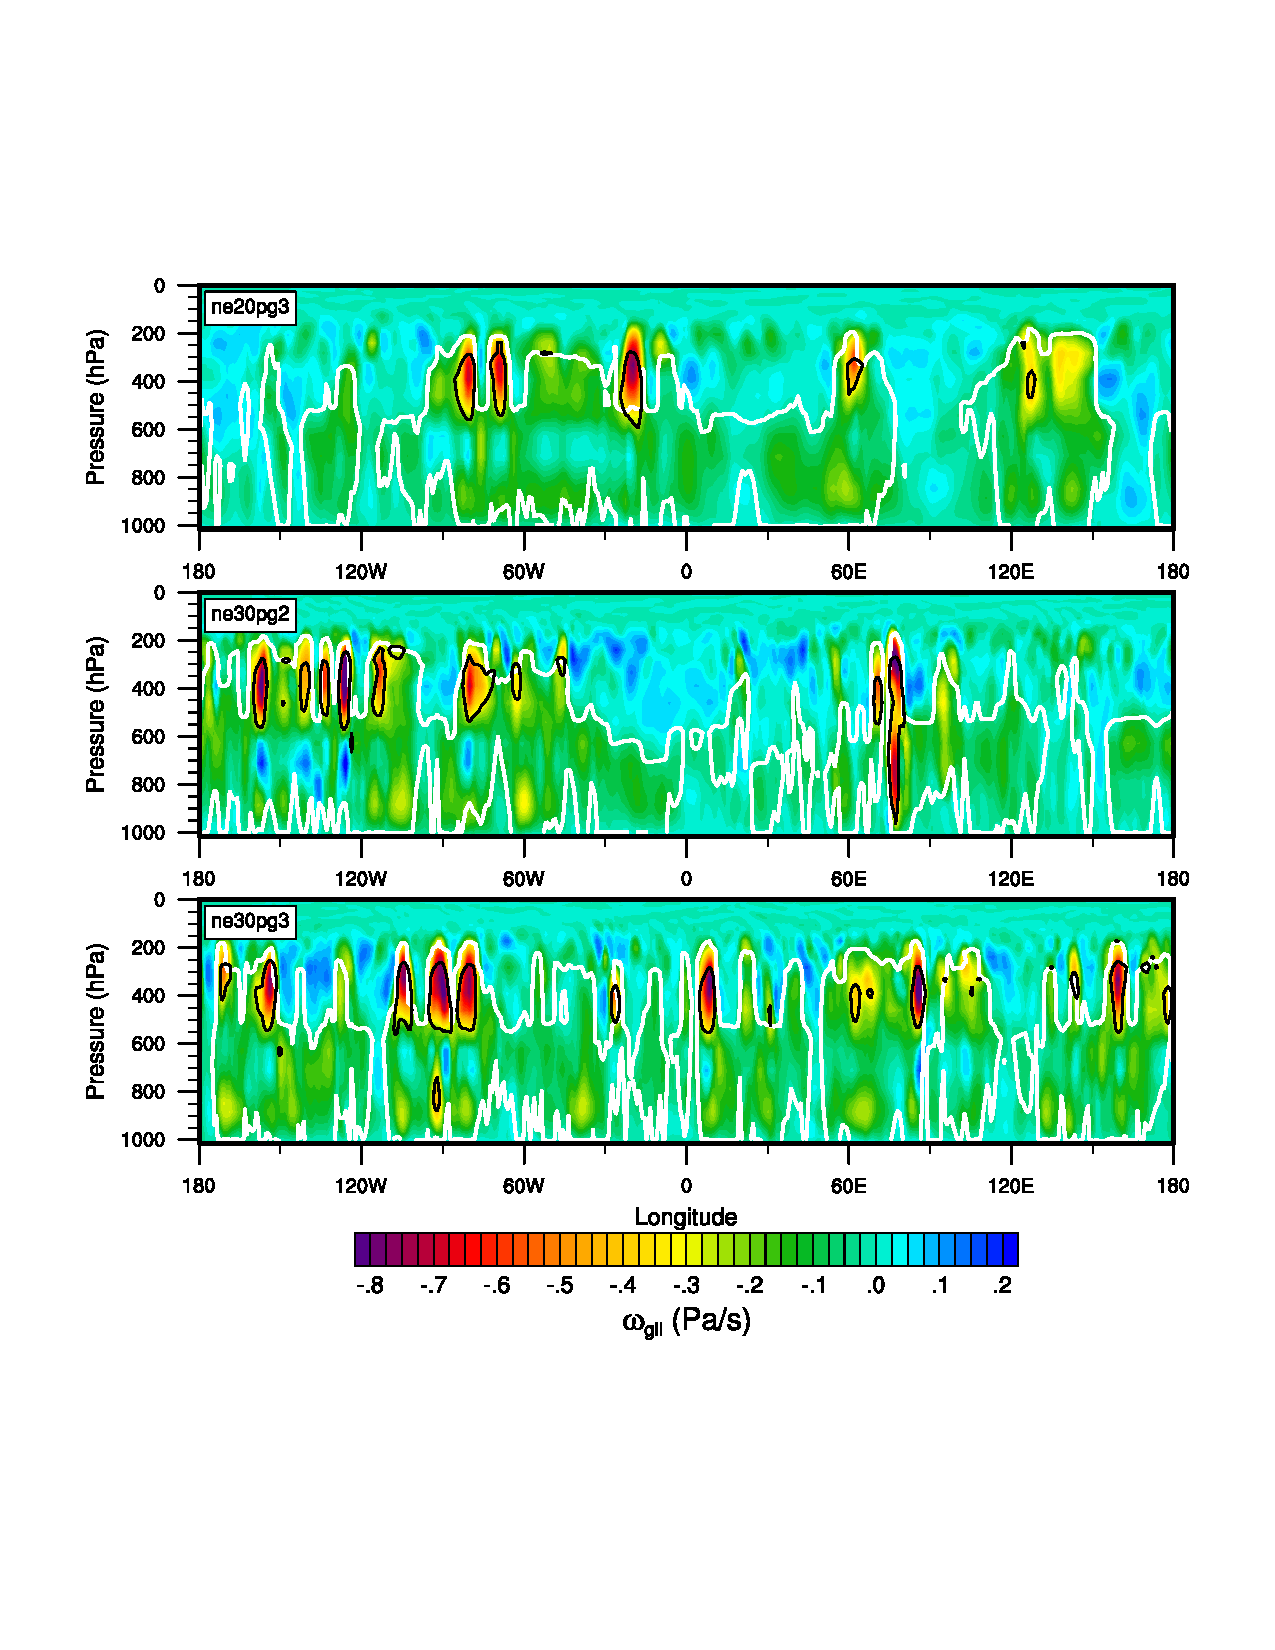
\includegraphics[width=30pc,angle=0]{figs/panel_transGLL.pdf}\\
\end{center}
\caption{Snapshots in the longitude-pressure plane of $\omega_{gll}$ through the ITCZ region in the $ne20pg3$, $ne30pg2$ and $ne30pg3$ configurations. Black is the $\pm 15 K/day$ contour of the physics tendencies, and the white contour is the $0.0075 kg/m^2/s$ contour of the parameterized deep convective mass fluxes.}
\label{fig:transx}
\end{figure}

It is not obvious from the snapshots in Figure~\ref{fig:transx} whether the characteristic length scale of the stratiform clouds, assumed here to be equal to the forcing scale, is any different across the three simulations. Analogous to determining the effective resolution \citep{S2011LNCSE}, the forcing scale may be inferred from the wave-number power spectrum of $f_T^{(gll)}$ as the maximum wavenumber prior to the steep, un-physical decline in power that characterizes the near-grid scale (hereafter $f_T^{(gll)}$ is referred to as the {\em{forcing}}). The wave-number power spectrum of the forcing in the middle-to-upper troposphere is shown in Figure~\ref{fig:pgXpanel-lores}a. Unlike kinetic energy spectra, the decline in forcing with wave-number is more gradual, making it difficult to determine a characteristic forcing scale from the spectra. However, it is clear that the slope of the $ne20pg3$ spectrum begins to steepen at smaller wavenumbers than in the $ne30pg3$ spectra. Additionally, the $ne30pg2$ spectra is remarkably similar to the $ne30pg3$ spectra, for all wavenumbers. These spectra indicate that the characteristic forcing scale in the $ne30pg2$ and $ne30pg3$ simulations are similar, and that both are smaller than the $ne20pg3$ forcing scale. From equation~\ref{eq:w-scale}, it is expected that the magnitude of the vertical motion is greater in both the $ne30pg2$ and $ne30pg3$ simulations.

\begin{figure}[t]
\begin{center}
\noindent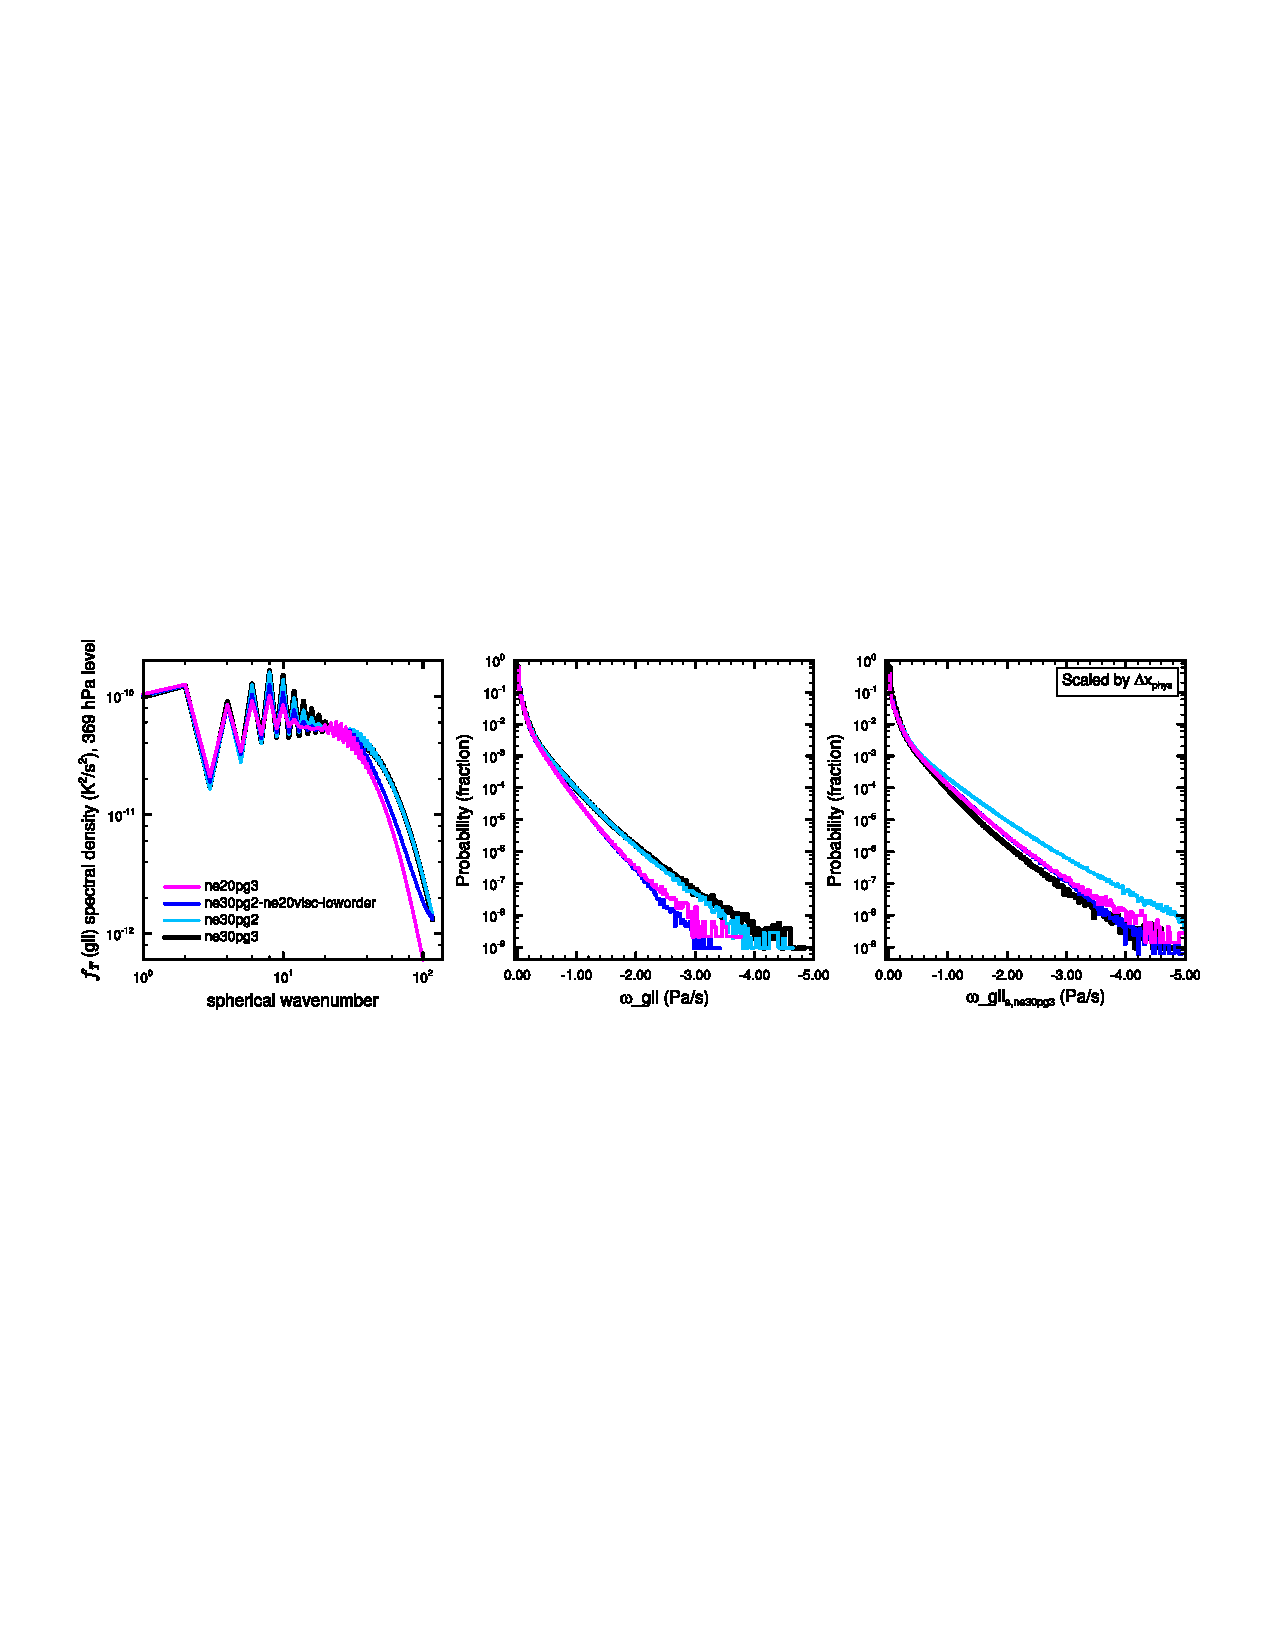
\includegraphics[width=30pc,angle=0]{figs/panel_ne20pg2-ne30pg2-ne30pg3.pdf}\\
\end{center}
\caption{(Left) Wavenumber-power spectrum of the temperature tendencies from the moist physics, near the 369 hPa level, (Middle) probability density distribution and (Right) the scaled probability density distribution of upward $\omega$ everywhere in the model. The scaled distributions are scaled to $ne30pg3$ using $\Delta x_{phys}$.}
\label{fig:pgXpanel-lores}
\end{figure}

The probability density function (PDF) of upward $\omega_{gll}$ everywhere in the simulations is shown in Figure~\ref{fig:pgXpanel-lores}b. Large magnitude $\omega_{gll}$ are more frequent in the $ne30pg2$ run, compared to $ne20pg3$, and the PDF is actually more similar to the $ne30pg3$ distribution, consistent with their similar forcing scales. This may be further illustrated through scaling the PDF's,
\begin{equation}
P_{s}(\omega) = \alpha \times P(\omega/\alpha),\label{eq:pdf}
\end{equation}
where $P_{s}(\omega)$ is the scaled PDF of $\omega$ and $\alpha$ is the ratio of $\omega$ to $\omega_{target}$, the $\omega$ associated with the target grid resolution, $\Delta x_{target}$. Making the assumption that the forcing scale is linear in $\Delta x$, then from equation~\ref{eq:w-scale}, $\alpha = \Delta x_{target}/\Delta x$. The target resolution is taken here to be equal to the $ne30pg3$ grid resolution. 

If the forcing scale of $ne30pg2$ is in fact determined by $\Delta x_{phys}$, then one sets $\Delta x = \Delta x_{phys}$ in $\alpha$. This scaled PDF, however, severely overestimates the frequency of upward $\omega$ of the target resolution, $ne30pg3$ (Figure~\ref{fig:pgXpanel-lores}c). It is clear from the similarity of the un-scaled PDF's of $ne30pg2$ and $ne30pg3$ (Figure~\ref{fig:pgXpanel-lores}b), and their forcing spectra (Figure~\ref{fig:pgXpanel-lores}a), that the forcing scale is determined by $\Delta x_{dyn}$, rather than $\Delta x_{phys}$. And one can be reasonably confident in the linear framework used to approximate $\alpha$ - the scaled $ne20pg3$ PDF fits the $ne30pg3$ distribution quite well. It then follows that the forcing scale of $ne20$ simulations is about $\frac{3}{2}$ times that of $ne30$ simulations, the ratio of their grid spacings.

There are two reasons the $pg2$ forcing scale is determined by the $GLL$ grid. The first being that the hyper-viscosity coefficients are a function of the $GLL$ grid resolution (equation~\ref{eq:hypervis}). The fourth-order hyper-viscosity is very scale-selective, targeting near grid-scale features more so than, e.g., a second-order operator. Despite this scale-selectiveness, the difference in $\Delta x_{phys}$ between $pg2$ and $pg3$ are small enough that the hyper-viscous smoothing render this distinction somewhat ambiguous, and the forcing scale is not all that sensitive to the coarser physics. This is illustrated through increasing $\nu$ in $ne30pg2$ to $ne20$ values, which causes the forcing to steepen at lower wavenumbers compared with the standard $ne30pg2$ run (not shown). However, the forcing still steepens at higher wavenumbers than in the $ne20pg3$ run (not shown), and so hyper-viscosity alone does not determine the forcing scale in $pg2$. In Appendix~\ref{sec:app2}, it is demonstrated that an additional factor is the use of high-order mapping of the forcing from the $pg2$ grid, to the $GLL$ and $CSLAM$ grids. High-order mapping in effect reconstructs scales that are not supported on the $pg2$ grid.

The combined effect of these two factors on the forcing scale is illustrated through an $ne30pg2$ simulation that uses low-order mapping (see Appendix~\ref{sec:app2}), and with hyper-viscosity coefficients set to $ne20$ values ($ne30pg2-ne20visc-loworder$ in Figure~\ref{fig:pgXpanel-lores}). The PDF of $\omega_{gll}$ and the forcing spectrum more closely resemble the $ne20pg3$ run. In this case, the forcing scale is more accurately determined by $\Delta x_{phys}$, since the scaled PDF is in fairly good agreement with the $ne30pg3$ simulation (Figure~\ref{fig:pgXpanel-lores}c).


\subsubsection{High Resolution}\label{sec:hires}

The experiment described in the previous section is repeated here for a $ne120pg2$ aqua-planet simulation, which corresponds to an approximate grid spacing of $\Delta x_{dyn} = 27.8km$ and $\Delta x_{phys} = 41.7km$. $ne80pg3$ refers to the grid in which the physics and dynamics are the same resolution as the physics of the $ne120pg2$ grid, and $ne120pg3$, the grid in which the physics and dynamics are equal to the resolution of the dynamics of $ne120pg2$. At these higher resolutions, the solutions are sensitive to $\Delta t_{phys}$ (Figure~\ref{fig:pdf-dtphys}), and so the $ne80$ grid uses a larger time-step than that of the $ne120$ grids (see Table~\ref{table:grids-hi}), following equation~\ref{eq:dt-scale}.

 \begin{table}
 \caption{$\Delta x$ and $\Delta t$ for the physics and dynamics in the high resolution simulations}
 \centering
 \begin{tabular}{llcccc}
 \hline
 Grid name & $\Delta x_{dyn}$  & $\Delta t_{dyn}$ & $\Delta x_{phys}$  & $\Delta t_{phys}$ \\
 \hline
   {\tt{ne}}80{\tt{pg3}}  & 41.7km & 112.5s  & 41.7km & 625s \\
   {\tt{ne}}120{\tt{pg2}}  & 27.8km & 75s  & 41.7km & 450s \\
   {\tt{ne}}120{\tt{pg3}}  & 27.8km & 75s  & 27.8km & 450s \\
 \hline
 \end{tabular}
 \label{table:grids-hi}
 \end{table}
 
 \begin{figure}[t]
\begin{center}
\noindent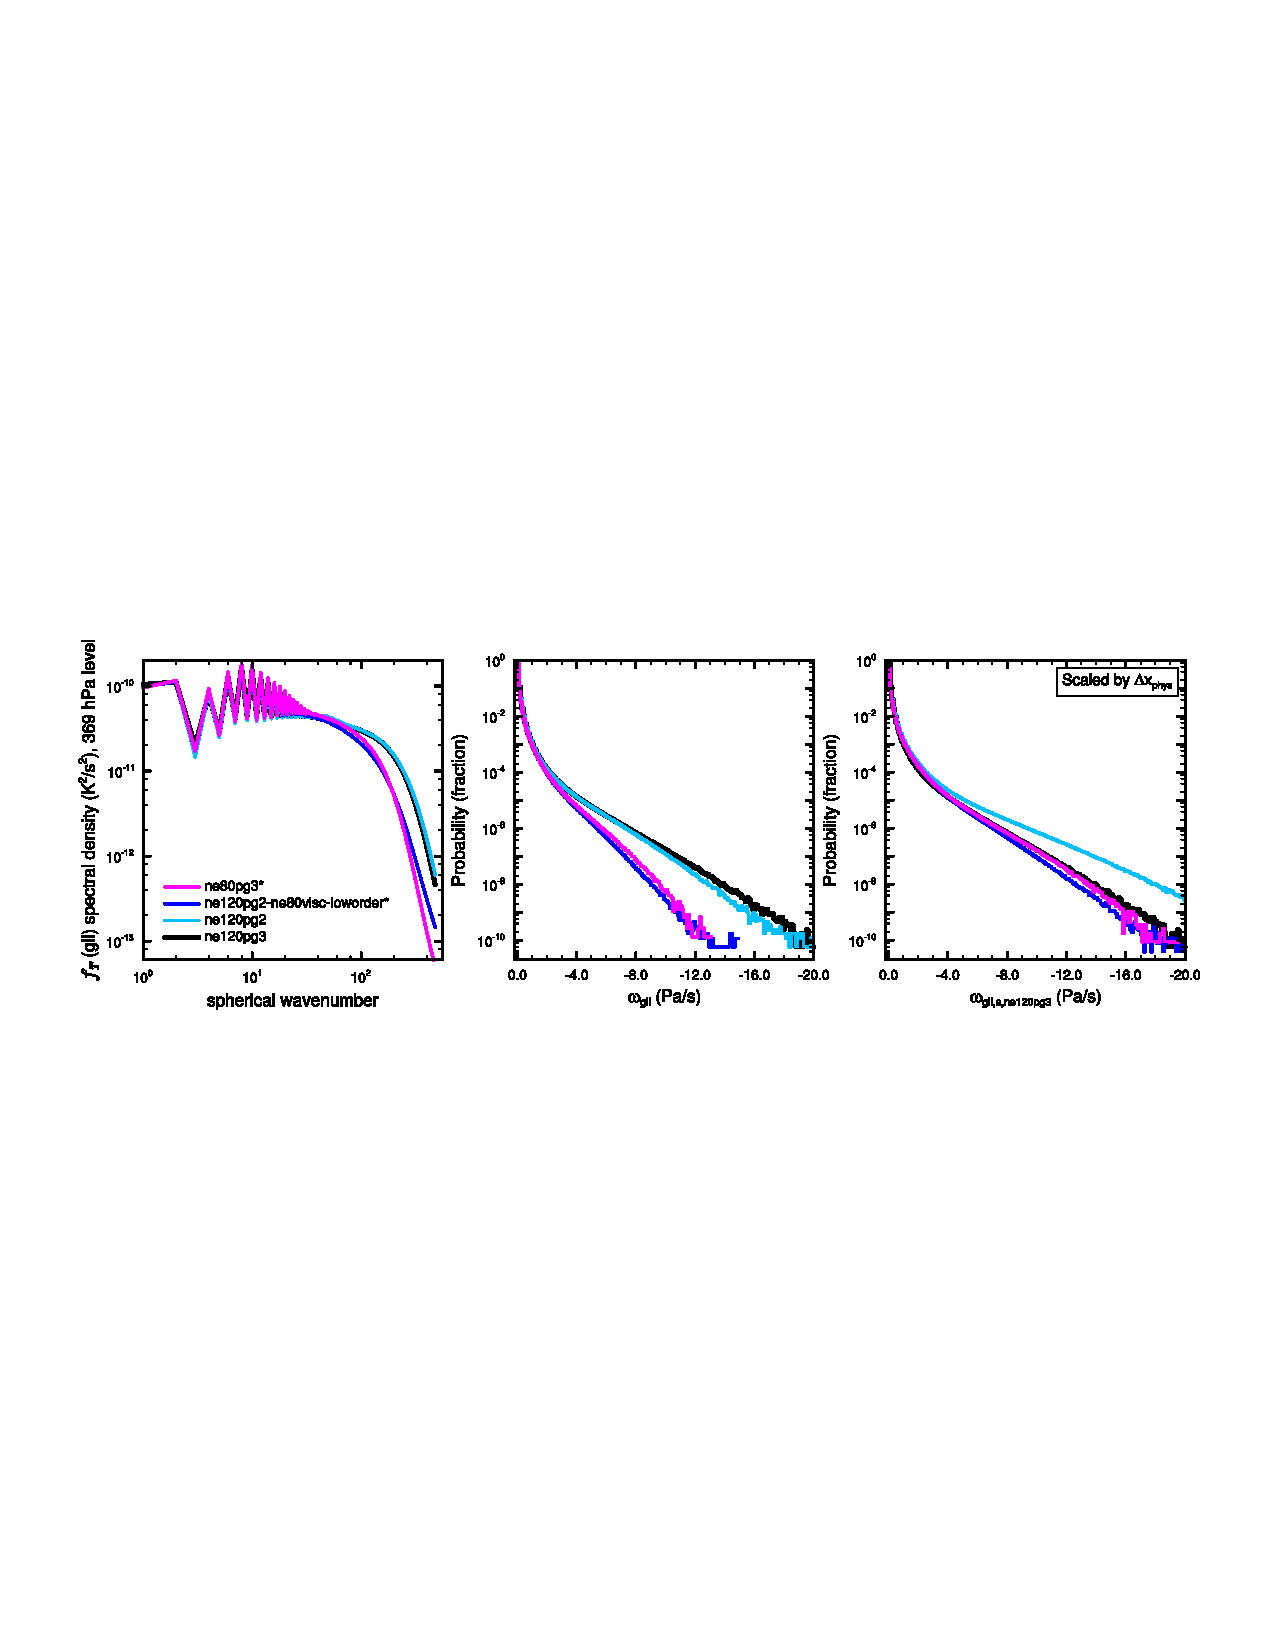
\includegraphics[width=30pc,angle=0]{figs/panel_ne80pg3_ne120pg2_ne120pg3.pdf}\\
\end{center}
\caption{As in Figure~\ref{fig:pgXpanel-lores}, but for the high resolution simulations. Asterisks indicate that $\Delta t_{phys}=675 s$, which is larger than that used for the default $ne120$ runs (see Table \ref{table:grids-hi}). {\color{red}{why is there so many spaces around the equal sign?}}}
\label{fig:pgXpanel-hires}
\end{figure}

Figure~\ref{fig:pgXpanel-hires} is the same as Figure~\ref{fig:pgXpanel-lores}, but for the high resolutions simulations. While the $ne80pg3$ forcing spectra begins to drop off just near wavenumber 100, the $ne120pg2$ and $ne120pg3$ drop off closer to wavenumber 200, and their spectra lie on top of one another (Figure~\ref{fig:pgXpanel-hires}a). The PDF's of (upward) $\omega_{gll}$ show that the $ne120$ distributions lie on top of one another, and while not a perfect match, both $ne120$ runs have substantially more frequent large magnitude vertical motion than in the $ne80pg3$ run (Figure~\ref{fig:pgXpanel-hires}b). As in the low resolution runs, the similarity of the $ne120$ forcing spectra and $\omega_{gll}$ distributions indicate that the forcing scale of the $ne120pg2$ run is not determined by the physics grid spacing, but rather the dynamics grid spacing. This is also evident from the over-prediction of the frequency of large magnitude $\omega_{gll}$ compared with the $ne120pg3$ run, through scaling the $ne120pg2$ PDF and setting the forcing scale proportional to $\Delta x_{phys}$ in equation~\ref{eq:pdf} (Figure~\ref{fig:pgXpanel-hires}c).

In the $ne120pg2$ simulation, the dynamics grid determines the forcing scale for the same two reasons found in the low resolution runs. The high-order mapping of the physics to the dynamics is important for reconstructing scales not supported on the $pg2$ grid, and scaling the viscosity coefficients by the dynamics grid spacing is also important. But in order to recreate the $ne80pg3$ solution using the $ne120pg2$ grid, the physics time-steps must be the same for these two grids. Combining all three modifications leads to an $ne120pg2$ solution that resembles the $ne80pg3$ run ($ne120pg2-ne80visc-loworder*$ in Figure~\ref{fig:pgXpanel-hires}). The forcing spectrum and distribution of $\omega_{gll}$ match that of the $ne80pg3$ run, and scaling the PDF by $\Delta x_{phys}$ closely resembles the $ne120pg3$ distribution.

\subsubsection{Across Resolutions}\label{sec:allres}

\begin{figure}[t]
\begin{center}
\noindent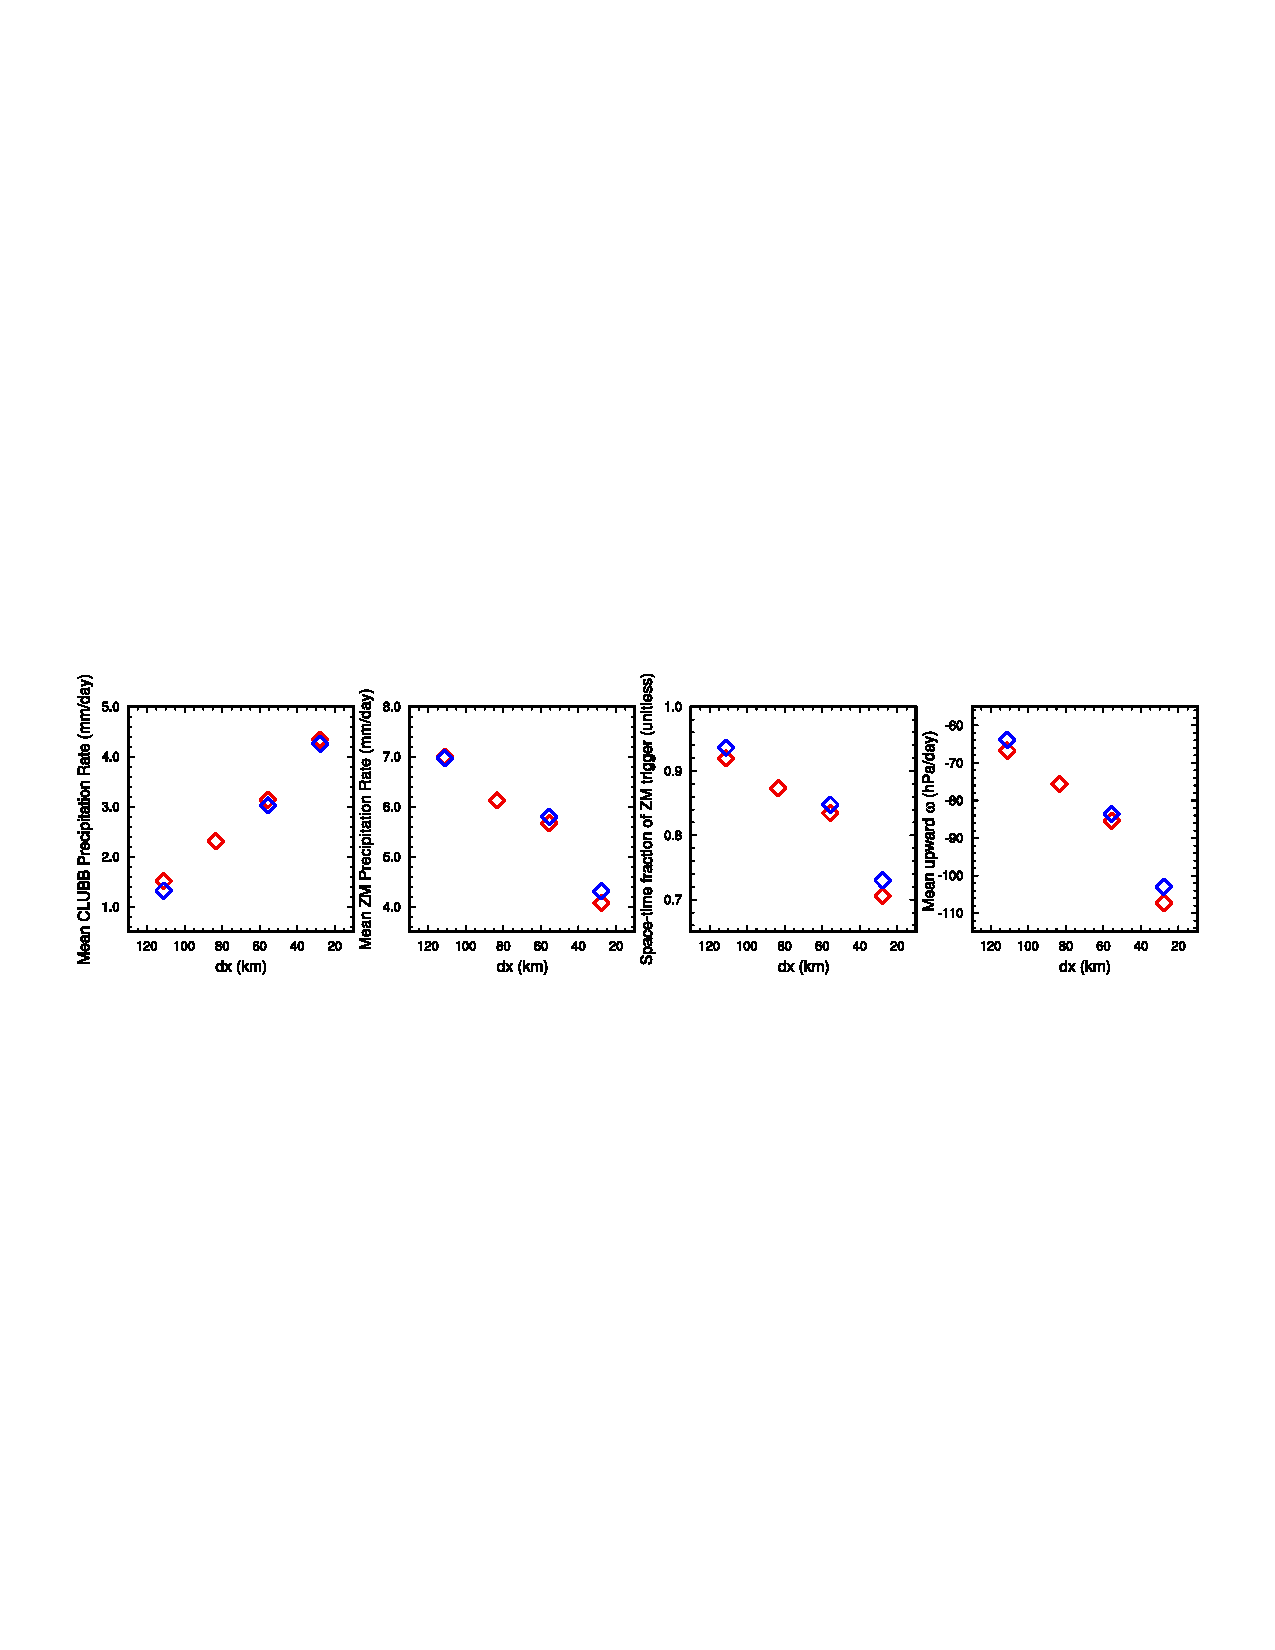
\includegraphics[width=30pc,angle=0]{figs/panel_diags.pdf}\\
\end{center}
\caption{Global mean, time-mean (a) upward $\omega$, (b) CLUBB precipitation rate and (c) parameterized deep convective precipitation rate. All means computed from the final 11 months of one-year simulations, and upward $\omega$ is computed using the corresponding 6-hourly output.}
\label{fig:diags}
\end{figure}

% \begin{table}
%\caption{Average equatorial grid spacing, $\Delta x$, and model time-step, $\Delta x$, used by the physical parameterizations, $phys$, and dynamical core, $dyn$.}
% \centering
%\begin{tabular}{llcccc}
%\hline
%Grid name & $\Delta x_{dyn}$  & $\Delta t_{dyn}$ & $\Delta x_{phys}$  & $\Delta t_{phys}$ \\
%\hline
% {\tt{ne}}40{\tt{pg3}}  &  83.4km & 150s  &  83.4km &  900s \\
% {\tt{ne}}60{\tt{pg2}}  &  55.6km & 150s  &  83.4km &  900s \\
%   {\tt{ne}}60{\tt{pg3}}  &  55.6km & 150s  &  55.6km &  900s \\
%   {\tt{ne}}80{\tt{pg3}}  &  41.7km &  75s  &  41.7km &  450s \\
%  {\tt{ne}}120{\tt{pg2}} &  27.8km &  75s  &  41.7km &  450s \\
%   {\tt{ne}}120{\tt{pg3}} &  27.8km &  75s  &  27.8km &  450s \\
%\hline
%\multicolumn{2}{l}{$^{a}$Footnote text here.}
%\end{tabular}
%\label{table:grids2}
%\end{table}

\section{Conclusions}\label{sec:conclusions}

Mitigating grid-imprinting through increasing the divergence damping coefficient an order of magnitude greater than is required for numerical stability is not ideal from a model development perspective. The hyper-viscosity coefficients are one of the only a handful of free-parameters in CAM-SE to tune the kinetic energy spectrum to match observations \citep{SPKS2014JAS,LetAl2018JAMES}. 

In sum, at low resolution, the default $pg2$ configuration does not degrade the resolution of the model since (1) the $GLL$ resolution is unchanged and (2) the high-order mapping is able to reproduce a state similar to what occurs in a $pg3$ configuration. Increasing the hyper-viscosity coefficients is akin to reducing the resolution of the $GLL$ solution.

%%

%  Numbered lines in equations:
%  To add line numbers to lines in equations,
%  \begin{linenomath*}
%  \begin{equation}
%  \end{equation}
%  \end{linenomath*}

%%% End of body of article

%%%%%%%%%%%%%%%%%%%%%%%%%%%%%%%%
%% Optional Appendix goes here
%
% The \appendix command resets counters and redefines section heads
%
% After typing \appendix
%
% will show
% A: Here Is Appendix Title
%
\appendix
\section{Defining $\Delta t_{phys}$ across resolutions}\label{sec:app1}
 \cite{HR2018JAMES} developed a moist bubble test, which indicate that time-truncation errors are large at high resolution (about $50km$ or less) using more conventional values for the physics time-step. The test may be able to provide incite on a reasonable scaling of $\Delta t_{phys}$ across resolutions in more complex configurations. In the test a set of non-rotating simulations are initialized with a warm, super-saturated moist bubble, and the grid spacing and bubble radius are simultaneously reduced by the same factor in each run through varying the planetary radius. The test was designed to mimic the reduction in buoyancy length scales that occur when the model resolution is increased in more complex configurations \citep{HETAL2006JCLIM,HR2018JAMES}. 
 
The moist bubble test is performed with CAM-SE-CSLAM and coupled to the simple condensation routine of \cite{K1969MM} across five different resolutions (pertaining to the $ne30$, $ne40$, $ne60$, $ne80$, and $ne120$ grids). The results are expressed as the minimum $\omega$ throughout each one day simulation, and shown in Figure~\ref{fig:bubble}. Two sets of simulations are performed with both $pg3$ and $pg2$, one with $\Delta t_{phys}$ determined by equation~\ref{eq:dt-scale}, and an equivalent set of simulations with $\Delta t_{phys} = 1800s$ for all resolutions. 

\begin{figure}[t]
\begin{center}
\noindent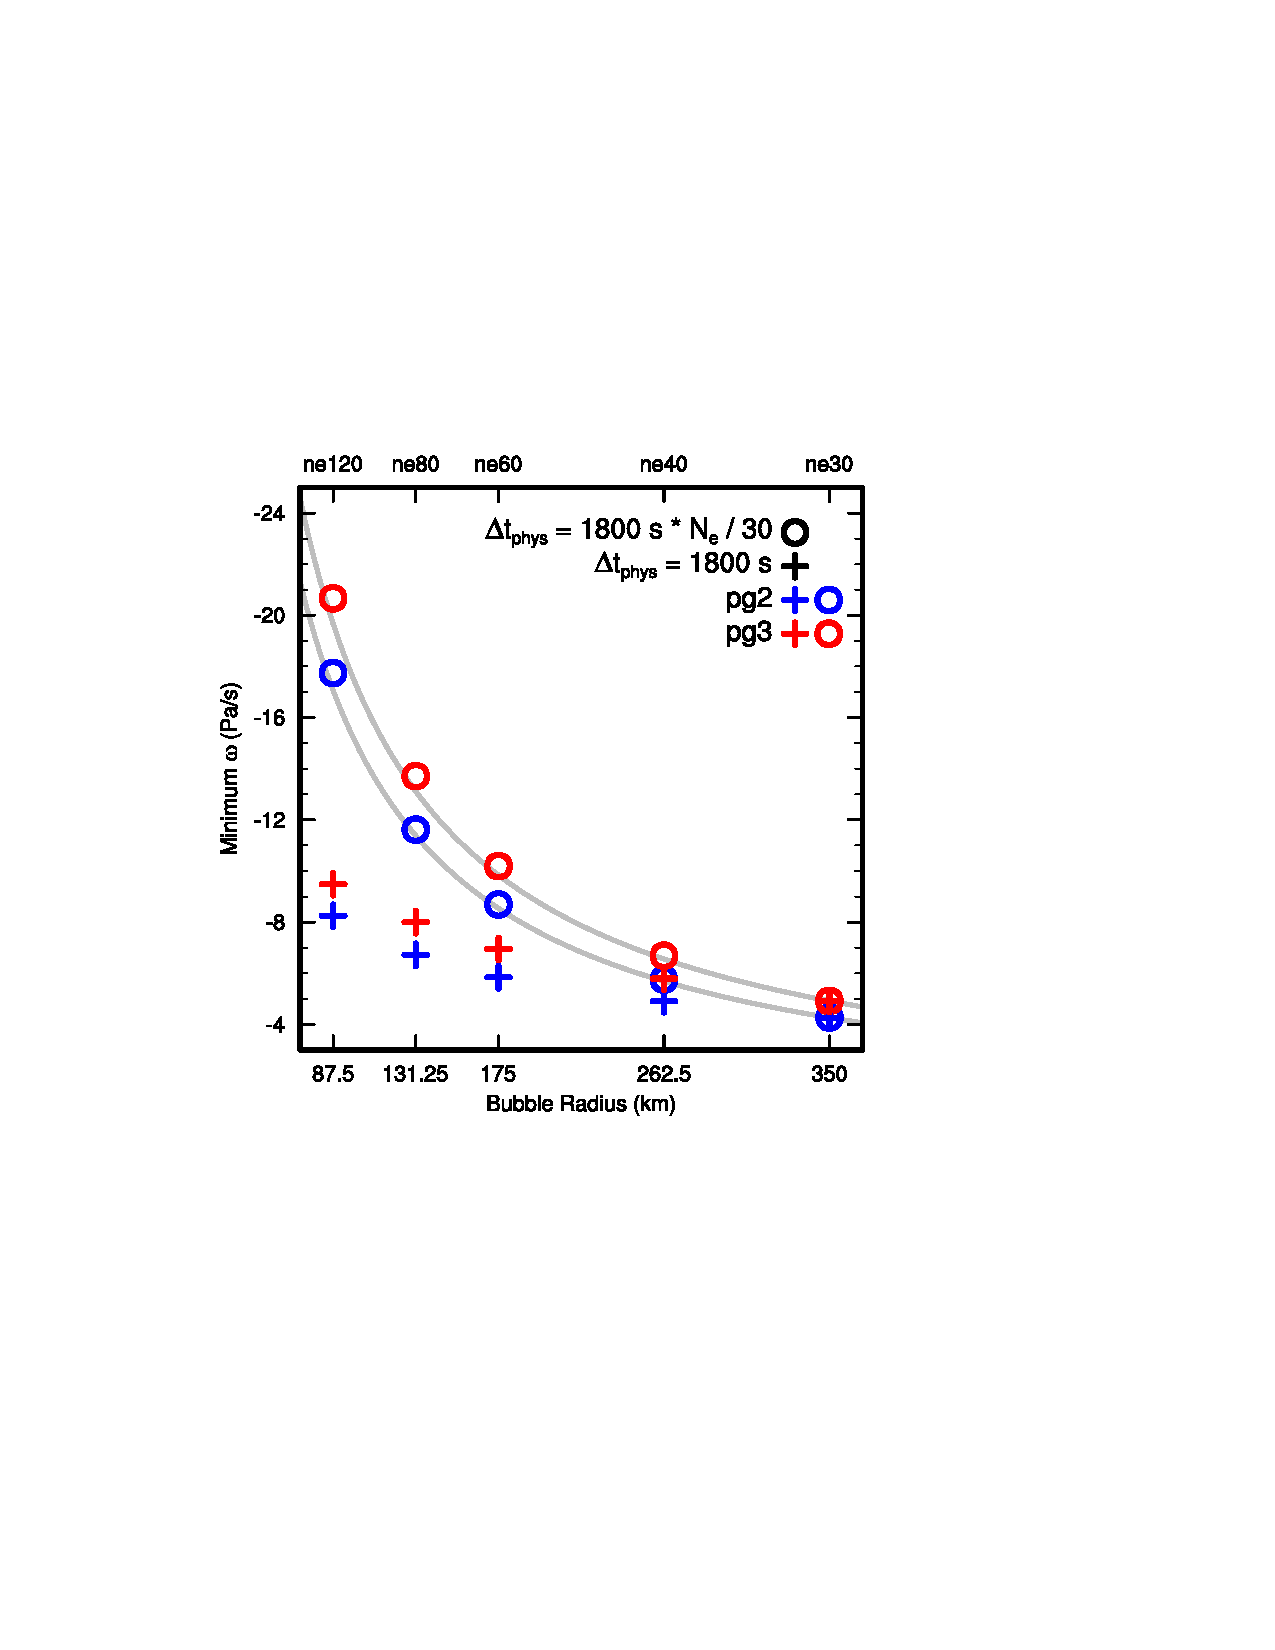
\includegraphics[width=25pc,angle=0]{figs/bubble_test.pdf}\\
\end{center}
\caption{The magnitude of $\omega$ in the $pg3$ solutions are systematically larger than the $pg2$ solutions, which is primarily a result of the damping effect of integrating the basis functions over a larger control volume.}
\label{fig:bubble}
\end{figure}

Since the diameters of the bubbles, $D$, are set proportional to $\Delta x_{dyn}$, \cite{HR2018JAMES} has shown that $\omega$ converges to the scaling of equation~\ref{eq:w-scale} in the limit of small $\Delta t_{phys}$, where small $\Delta t_{phys}$ refers to the CFL limiting time-step used by the dynamics. Equation~\ref{eq:w-scale} is overlain as grey lines in Figure~\ref{fig:bubble}, with $ne30$ being the reference resolution. The solutions using $\Delta t_{phys}$ from equation~\ref{eq:dt-scale} follow the scaling, whereas fixing $\Delta t_{phys} = 1800s$ across resolutions damps the solution relative to the analytical solution, progressively more so at higher resolutions. If $\Delta t_{phys}$ is too large, the solution has non-negligible error, which is avoided through scaling $\Delta t_{phys}$ according to equation~\ref{eq:dt-scale}.

To get a a handle on whether the test is useful for understanding more realistic configurations, four aqua-planet simulations are performed using the CAM6 physics package. A pair of $ne30pg2$ simulations, one in which $\Delta t_{phys}$ is set to the appropriate value from equation~\ref{eq:dt-scale} ($1800s$), and another where it is set to the $\Delta t_{phys}$ corresponding to the $ne20$ resolution ($2700s$). Similarly, a pair of $ne120pg2$ simulations are performed, one with $\Delta t_{phys}$ set to the value from equation~\ref{eq:dt-scale} ($450s$), and one with $\Delta t_{phys}$ set to the $ne80$ value ($625s$). 

\begin{figure}[t]
\begin{center}
\noindent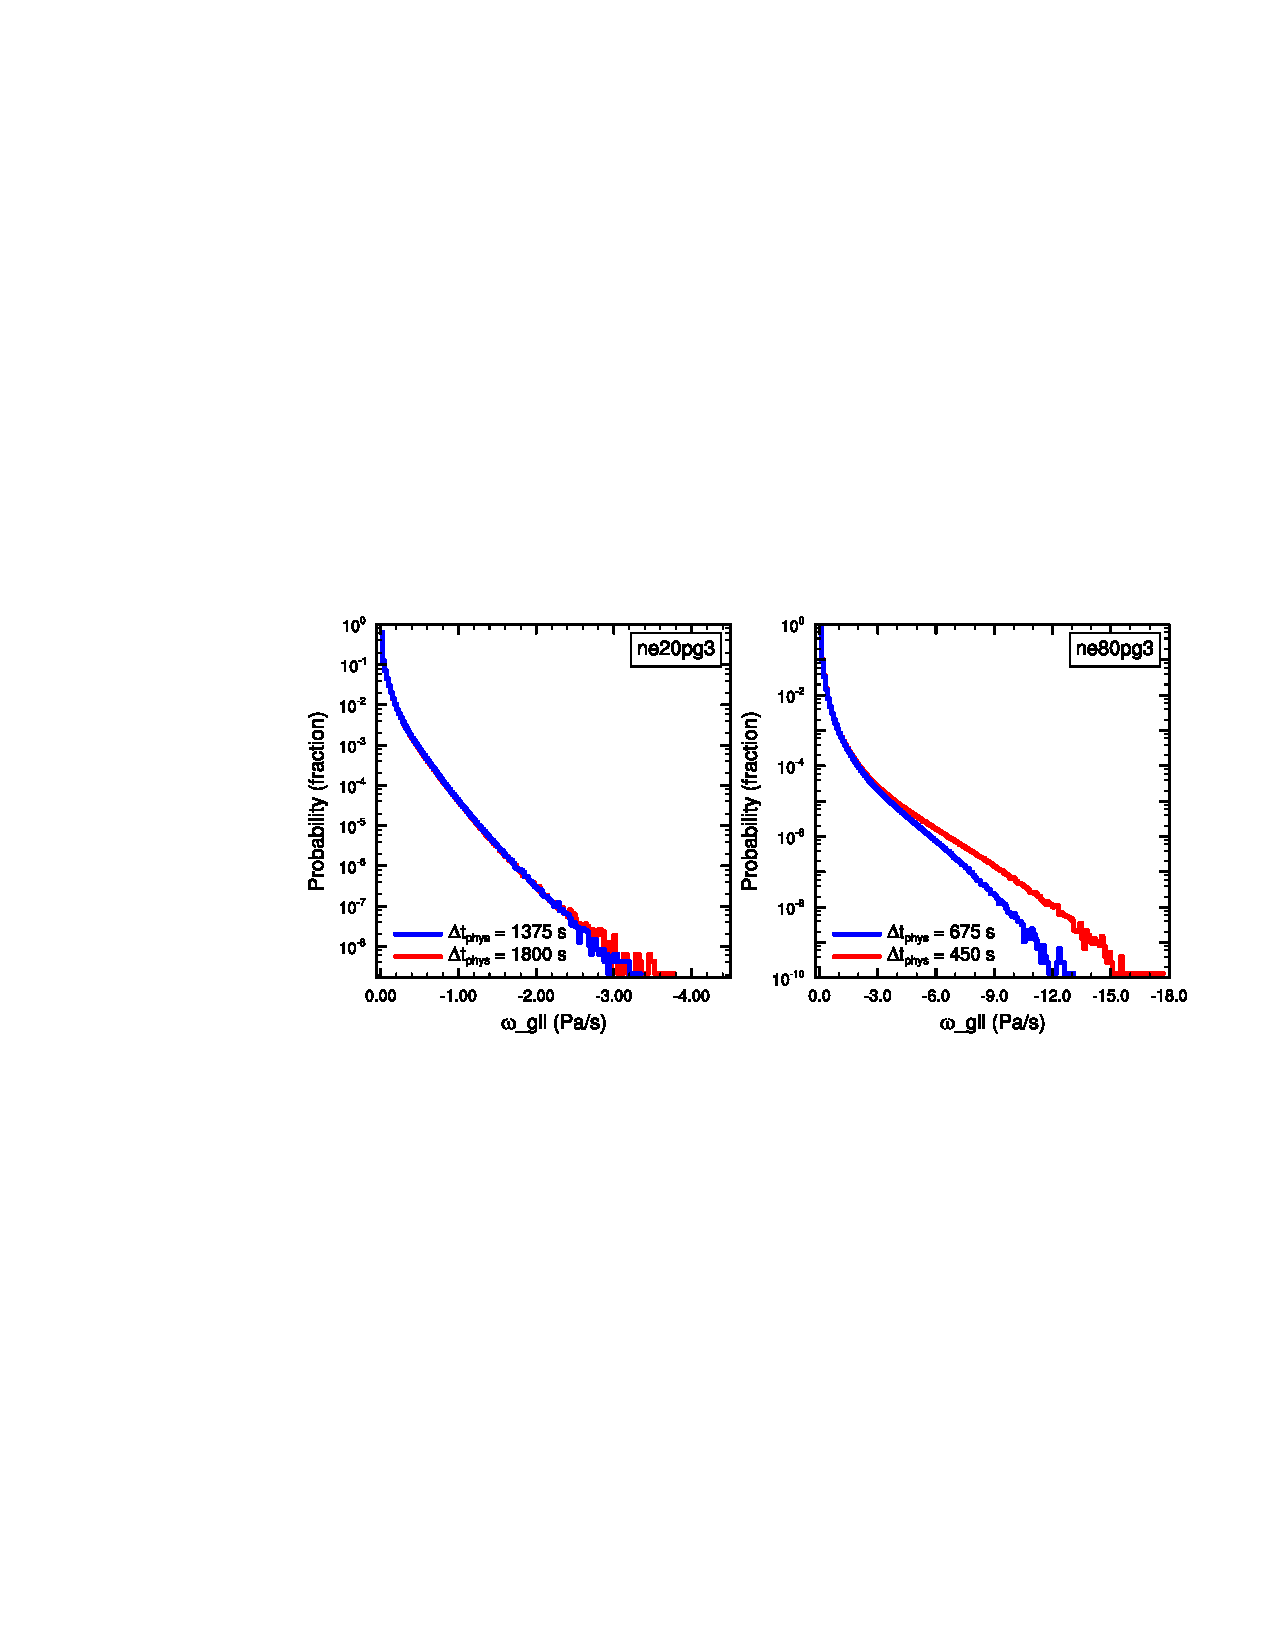
\includegraphics[width=30pc,angle=0]{figs/panel_pdf_dtphys.pdf}\\
\end{center}
\caption{Probability density distribution of upward $\omega$ everywhere in the model in the aqua-planets using the $ne30pg2$ grid (Left) and the $ne120pg2$ grid (Right). Figure computed for one year of 6-hourly data. The different colors indicate the physics time-steps used in the runs.}
\label{fig:pdf-dtphys}
\end{figure}

Figure~\ref{fig:pdf-dtphys} shows the PDFs of upward $\omega$ computed from a year of six-hourly data in the simulations. At lower resolution, $\Delta t_{phys}$ has only a very small effect on the solution, near the tale-end of the distributions. At high-resolution, values of $\omega$ less then about $3 Pa/s$ are more frequent in the small $\Delta t_{phys}$ run, with the discrepancy growing more for larger magnitudes of $\omega$. The progressively larger errors with increasing resolution also manifests in the moist bubble tests, indicating that truncation errors arising from large $\Delta t_{phys}$ do exist in more complex configurations.

\section{The impact of high-order mapping to the dynamics grids}\label{sec:app2}

Figure~\ref{fig:loworder}a shows a close-up of the wavenumber power spectrum of the forcing on the $pg$ grid (dotted), where it is computed, and on the $GLL$ grid (solid), where it is has been mapped. In $ne30pg3$, the magnitudes are similar on both grids, except the mapping tends to damp the high wavenumbers of the forcing on the $GLL$ grid (greater than 60), but these scales are primarily below the effective resolution of the model and should not effect the solution. For $ne30pg2$, the magnitude of the forcing is actually greater after mapping to the $GLL$ grid, and more similar to the forcing in the $ne30pg3$ simulations. The high-order mapping can therefore replicate the scales of the physics tendencies that occur in the $pg3$ simulation, even though the physics are evaluated on a coarser $pg2$ grid.

\begin{figure}[t]
\begin{center}
\noindent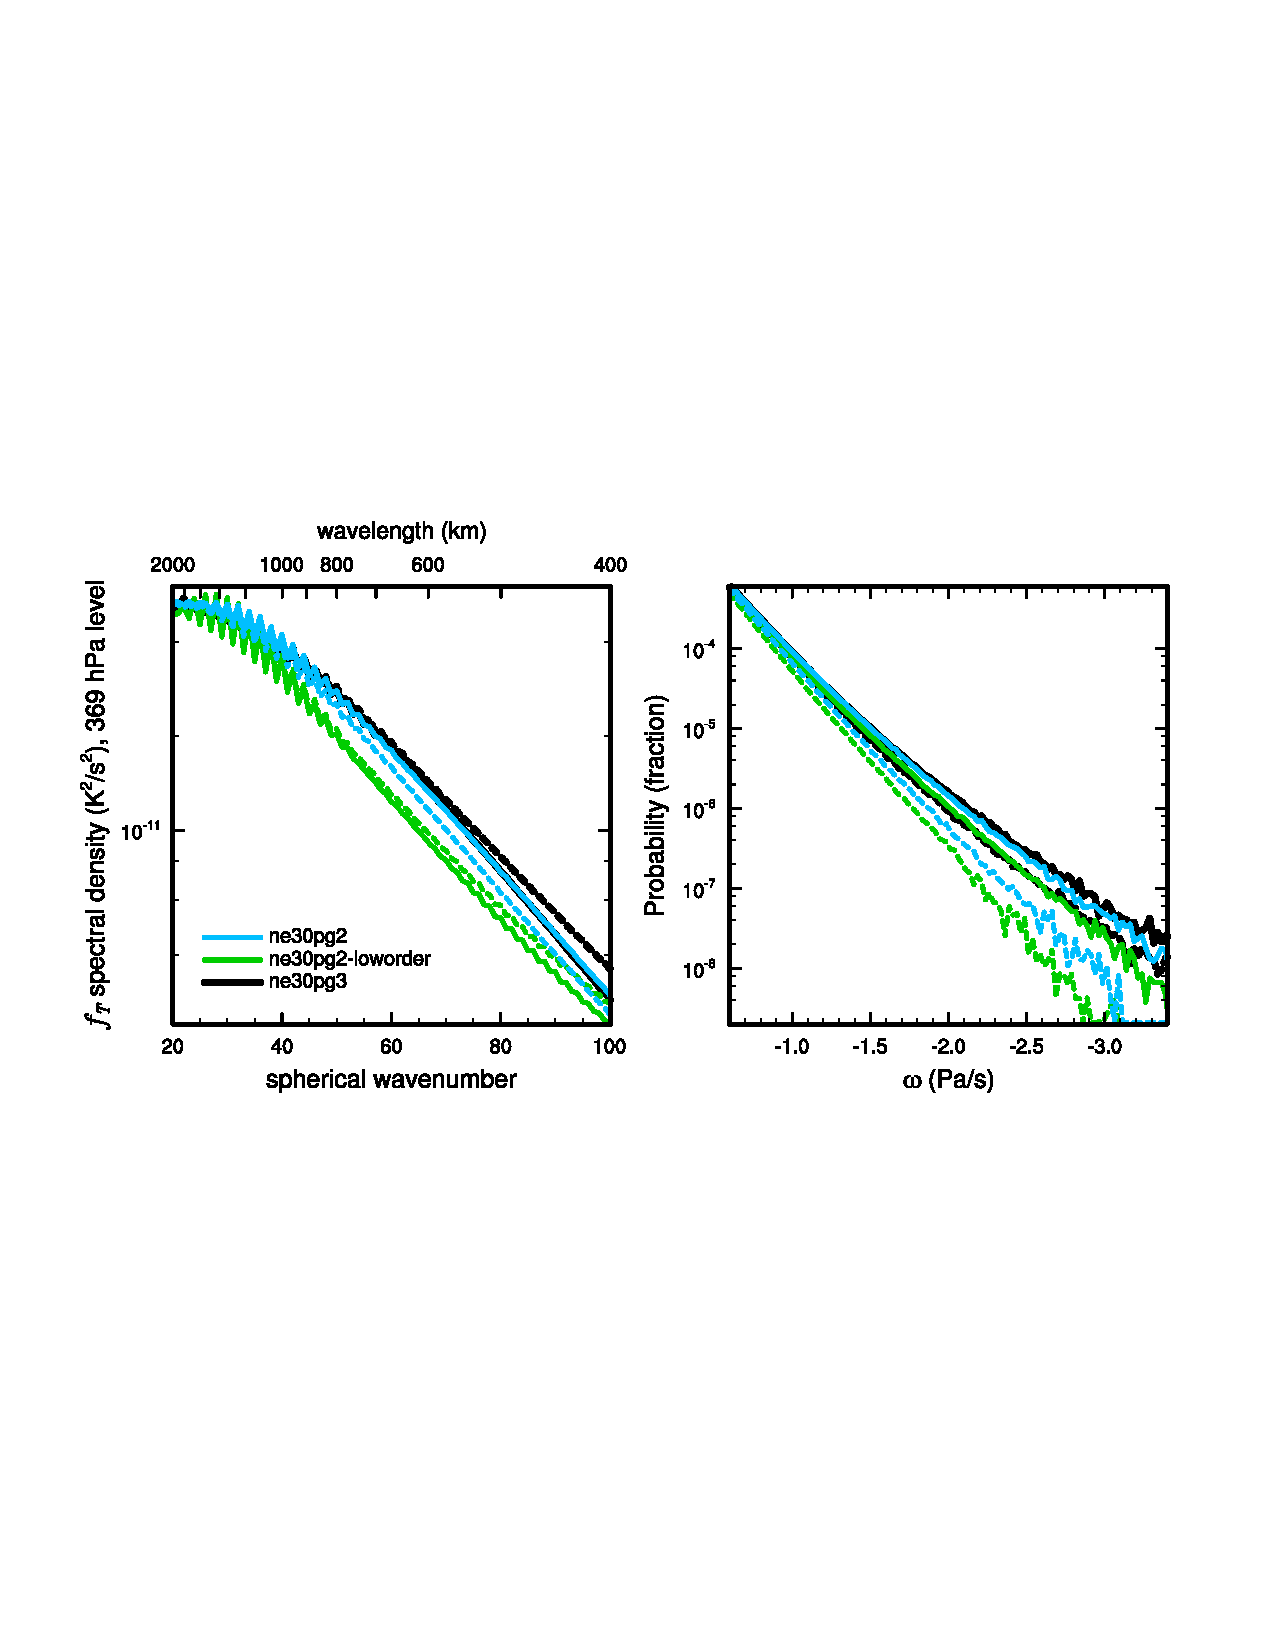
\includegraphics[width=30pc,angle=0]{figs/panel_loworder.pdf}\\
\end{center}
\caption{(Left) Wavenumber-power spectrum of the temperature tendencies from the moist physics, at the 369 hPa level, and (right) probability density distribution of upward $\omega$, everywhere in the model, for three year-long aqua-planet simulations. Solid lines refer to values of on the $GLL$ grids, and dashed lines, the fields on the $pg$ grids. See text for details regarding the three simulations.}
\label{fig:loworder}
\end{figure}

The importance of the high-order mapping can be shown with an additional $ne30pg2$ simulation, using low-order mapping ($ne30pg2-loworder$ in Figure~\ref{fig:loworder}). Specifically, low-order mapping refers to piecewise constant mapping from $pg2$ to $CSLAM$ and bi-linear mapping from $pg2$ to $GLL$. The forcing spectrum is now similar on both the $pg2$ and $GLL$ grids, although the low-order mapping tends to damp the forcing on the $GLL$ grid for wavenumbers greater than about 60, scales below than the effective resolution (Figure~\ref{fig:loworder}a). A close up of the PDF of $\omega_{gll}$ is provided in Figure~\ref{fig:loworder}b (solid lines). As expected, the frequency of large magnitude $\omega_{gll}$ in the low-order run is less compared to the default $ne30pg2$ simulation. 

The dotted lines in Figure~\ref{fig:loworder}b show the PDF of $\omega$ on the $pg$ grids. The frequency of large magnitude $\omega$ is reduced on the $pg$ grids, compared to the state on the $GLL$ grids. This is primarily due to the smoothing effect of integrating the nodal point values over control volumes (H18). The larger $\omega$ values are even less frequent on the $pg2$ grid due to integrating over control volumes $\frac{9}{4}$ times greater than the $pg3$ control volumes. 


%%%%%%%%%%%%%%%%%%%%%%%%%%%%%%%%%%%%%%%%%%%%%%%%%%%%%%%%%%%%%%%%
%
%  ACKNOWLEDGMENTS
%
% The acknowledgments must list:
%
% •	All funding sources related to this work from all authors
%
% •	Any real or perceived financial conflicts of interests for any
%	author
%
% •	Other affiliations for any author that may be perceived as
% 	having a conflict of interest with respect to the results of this
% 	paper.
%
% •	A statement that indicates to the reader where the data
% 	supporting the conclusions can be obtained (for example, in the
% 	references, tables, supporting information, and other databases).
%
% It is also the appropriate place to thank colleagues and other contributors. 
% AGU does not normally allow dedications.

%\acknowledgments

%% ------------------------------------------------------------------------ %%
%% Citations

% Please use ONLY \citet and \citep for reference citations.
% DO NOT use other cite commands (e.g., \cite, \citeyear, \nocite, \citealp, etc.).


%% Example \citet and \citep:
%  ...as shown by \citet{Boug10}, \citet{Buiz07}, \citet{Fra10},
%  \citet{Ghel00}, and \citet{Leit74}. 

%  ...as shown by \citep{Boug10}, \citep{Buiz07}, \citep{Fra10},
%  \citep{Ghel00, Leit74}. 

%  ...has been shown \citep [e.g.,][]{Boug10,Buiz07,Fra10}.



%%  REFERENCE LIST AND TEXT CITATIONS
%
% Either type in your references using
%
% \begin{theliography}{}
% \bibitem[{\textit{Kobayashi et~al.}}(2003)]{R2013} Kobayashi, T.,
% Tran, A.~H., Nishijo, H., Ono, T., and Matsumoto, G.  (2003).
% Contribution of hippocampal place cell activity to learning and
% formation of goal-directed navigation in rats. \textit{Neuroscience}
% 117, 1025--1035.
%
% \bibitem{}
% Text
% \end{thebibliography}
%
\bibliography{bib}
%%%%%%%%%%%%%%%%%%%%%%%%%%%%%%%%%%%%%%%%%%%%%%%
% Or, to use BibTeX:
%
% Follow these steps
%
% 1. Type in \bibliography{<name of your .bib file>} 
%    Run LaTeX on your LaTeX file.
%
% 2. Run BiBTeX on your LaTeX file.
%
% 3. Open the new .bbl file containing the reference list and
%   copy all the contents into your LaTeX file here.
%
% 4. Run LaTeX on your new file which will produce the citations.
%
% AGU does not want a .bib or a .bbl file. Please copy in the contents of your .bbl file here.


%% After you run BibTeX, Copy in the contents of the .bbl file here:


%%%%%%%%%%%%%%%%%%%%%%%%%%%%%%%%%%%%%%%%%%%%%%%%%%%%%%%%%%%%%%%%%%%%%
% Track Changes:
% To add words, \added{<word added>}
% To delete words, \deleted{<word deleted>}
% To replace words, \replace{<word to be replaced>}{<replacement word>}
% To explain why change was made: \explain{<explanation>} This will put
% a comment into the right margin.

%%%%%%%%%%%%%%%%%%%%%%%%%%%%%%%%%%%%%%%%%%%%%%%%%%%%%%%%%%%%%%%%%%%%%
% At the end of the document, use \listofchanges, which will list the
% changes and the page and line number where the change was made.

% When final version, \listofchanges will not produce anything,
% \added{<word or words>} word will be printed, \deleted{<word or words} will take away the word,
% \replaced{<delete this word>}{<replace with this word>} will print only the replacement word.
%  In the final version, \explain will not print anything.
%%%%%%%%%%%%%%%%%%%%%%%%%%%%%%%%%%%%%%%%%%%%%%%%%%%%%%%%%%%%%%%%%%%%%

%%%
\listofchanges
%%%

\end{document}

%%%%%%%%%%%%%%%%%%%%%%%%%%%%%%%%%%%%%
%% Supporting Information
%% (Optional) See AGUSuppInfoSamp.tex/pdf for requirements 
%% for Supporting Information.
%%%%%%%%%%%%%%%%%%%%%%%%%%%%%%%%%%%%%



%%%%%%%%%%%%%%%%%%%%%%%%%%%%%%%%%%%%%%%%%%%%%%%%%%%%%%%%%%%%%%%

More Information and Advice:

%% ------------------------------------------------------------------------ %%
%
%  SECTION HEADS
%
%% ------------------------------------------------------------------------ %%

% Capitalize the first letter of each word (except for
% prepositions, conjunctions, and articles that are
% three or fewer letters).

% AGU follows standard outline style; therefore, there cannot be a section 1 without
% a section 2, or a section 2.3.1 without a section 2.3.2.
% Please make sure your section numbers are balanced.
% ---------------
% Level 1 head
%
% Use the \section{} command to identify level 1 heads;
% type the appropriate head wording between the curly
% brackets, as shown below.
%
%An example:
%\section{Level 1 Head: Introduction}
%
% ---------------
% Level 2 head
%
% Use the \subsection{} command to identify level 2 heads.
%An example:
%\subsection{Level 2 Head}
%
% ---------------
% Level 3 head
%
% Use the \subsubsection{} command to identify level 3 heads
%An example:
%\subsubsection{Level 3 Head}
%
%---------------
% Level 4 head
%
% Use the \subsubsubsection{} command to identify level 3 heads
% An example:
%\subsubsubsection{Level 4 Head} An example.
%
%% ------------------------------------------------------------------------ %%
%
%  IN-TEXT LISTS
%
%% ------------------------------------------------------------------------ %%
%
% Do not use bulleted lists; enumerated lists are okay.
% \begin{enumerate}
% \item
% \item
% \item
% \end{enumerate}
%
%% ------------------------------------------------------------------------ %%
%
%  EQUATIONS
%
%% ------------------------------------------------------------------------ %%

% Single-line equations are centered.
% Equation arrays will appear left-aligned.

Math coded inside display math mode \[ ...\]
 will not be numbered, e.g.,:
 \[ x^2=y^2 + z^2\]

 Math coded inside \begin{equation} and \end{equation} will
 be automatically numbered, e.g.,:
 \begin{equation}
 x^2=y^2 + z^2
 \end{equation}


% To create multiline equations, use the
% \begin{eqnarray} and \end{eqnarray} environment
% as demonstrated below.
\begin{eqnarray}
  x_{1} & = & (x - x_{0}) \cos \Theta \nonumber \\
        && + (y - y_{0}) \sin \Theta  \nonumber \\
  y_{1} & = & -(x - x_{0}) \sin \Theta \nonumber \\
        && + (y - y_{0}) \cos \Theta.
\end{eqnarray}

%If you don't want an equation number, use the star form:
%\begin{eqnarray*}...\end{eqnarray*}

% Break each line at a sign of operation
% (+, -, etc.) if possible, with the sign of operation
% on the new line.

% Indent second and subsequent lines to align with
% the first character following the equal sign on the
% first line.

% Use an \hspace{} command to insert horizontal space
% into your equation if necessary. Place an appropriate
% unit of measure between the curly braces, e.g.
% \hspace{1in}; you may have to experiment to achieve
% the correct amount of space.


%% ------------------------------------------------------------------------ %%
%
%  EQUATION NUMBERING: COUNTER
%
%% ------------------------------------------------------------------------ %%

% You may change equation numbering by resetting
% the equation counter or by explicitly numbering
% an equation.

% To explicitly number an equation, type \eqnum{}
% (with the desired number between the brackets)
% after the \begin{equation} or \begin{eqnarray}
% command.  The \eqnum{} command will affect only
% the equation it appears with; LaTeX will number
% any equations appearing later in the manuscript
% according to the equation counter.
%

% If you have a multiline equation that needs only
% one equation number, use a \nonumber command in
% front of the double backslashes (\\) as shown in
% the multiline equation above.

% If you are using line numbers, remember to surround
% equations with \begin{linenomath*}...\end{linenomath*}

%  To add line numbers to lines in equations:
%  \begin{linenomath*}
%  \begin{equation}
%  \end{equation}
%  \end{linenomath*}



